\documentclass[twoside]{book}

% Packages required by doxygen
\usepackage{fixltx2e}
\usepackage{calc}
\usepackage{doxygen}
\usepackage[export]{adjustbox} % also loads graphicx
\usepackage{graphicx}
\usepackage[utf8]{inputenc}
\usepackage{makeidx}
\usepackage{multicol}
\usepackage{multirow}
\PassOptionsToPackage{warn}{textcomp}
\usepackage{textcomp}
\usepackage[nointegrals]{wasysym}
\usepackage[table]{xcolor}

% Font selection
\usepackage[T1]{fontenc}
\usepackage[scaled=.90]{helvet}
\usepackage{courier}
\usepackage{amssymb}
\usepackage{sectsty}
\renewcommand{\familydefault}{\sfdefault}
\allsectionsfont{%
  \fontseries{bc}\selectfont%
  \color{darkgray}%
}
\renewcommand{\DoxyLabelFont}{%
  \fontseries{bc}\selectfont%
  \color{darkgray}%
}
\newcommand{\+}{\discretionary{\mbox{\scriptsize$\hookleftarrow$}}{}{}}

% Page & text layout
\usepackage{geometry}
\geometry{%
  a4paper,%
  top=2.5cm,%
  bottom=2.5cm,%
  left=2.5cm,%
  right=2.5cm%
}
\tolerance=750
\hfuzz=15pt
\hbadness=750
\setlength{\emergencystretch}{15pt}
\setlength{\parindent}{0cm}
\setlength{\parskip}{3ex plus 2ex minus 2ex}
\makeatletter
\renewcommand{\paragraph}{%
  \@startsection{paragraph}{4}{0ex}{-1.0ex}{1.0ex}{%
    \normalfont\normalsize\bfseries\SS@parafont%
  }%
}
\renewcommand{\subparagraph}{%
  \@startsection{subparagraph}{5}{0ex}{-1.0ex}{1.0ex}{%
    \normalfont\normalsize\bfseries\SS@subparafont%
  }%
}
\makeatother

% Headers & footers
\usepackage{fancyhdr}
\pagestyle{fancyplain}
\fancyhead[LE]{\fancyplain{}{\bfseries\thepage}}
\fancyhead[CE]{\fancyplain{}{}}
\fancyhead[RE]{\fancyplain{}{\bfseries\leftmark}}
\fancyhead[LO]{\fancyplain{}{\bfseries\rightmark}}
\fancyhead[CO]{\fancyplain{}{}}
\fancyhead[RO]{\fancyplain{}{\bfseries\thepage}}
\fancyfoot[LE]{\fancyplain{}{}}
\fancyfoot[CE]{\fancyplain{}{}}
\fancyfoot[RE]{\fancyplain{}{\bfseries\scriptsize Generated by Doxygen }}
\fancyfoot[LO]{\fancyplain{}{\bfseries\scriptsize Generated by Doxygen }}
\fancyfoot[CO]{\fancyplain{}{}}
\fancyfoot[RO]{\fancyplain{}{}}
\renewcommand{\footrulewidth}{0.4pt}
\renewcommand{\chaptermark}[1]{%
  \markboth{#1}{}%
}
\renewcommand{\sectionmark}[1]{%
  \markright{\thesection\ #1}%
}

% Indices & bibliography
\usepackage{natbib}
\usepackage[titles]{tocloft}
\setcounter{tocdepth}{3}
\setcounter{secnumdepth}{5}
\makeindex

% Hyperlinks (required, but should be loaded last)
\usepackage{ifpdf}
\ifpdf
  \usepackage[pdftex,pagebackref=true]{hyperref}
\else
  \usepackage[ps2pdf,pagebackref=true]{hyperref}
\fi
\hypersetup{%
  colorlinks=true,%
  linkcolor=blue,%
  citecolor=blue,%
  unicode%
}

% Custom commands
\newcommand{\clearemptydoublepage}{%
  \newpage{\pagestyle{empty}\cleardoublepage}%
}

\usepackage{caption}
\captionsetup{labelsep=space,justification=centering,font={bf},singlelinecheck=off,skip=4pt,position=top}

%===== C O N T E N T S =====

\begin{document}

% Titlepage & ToC
\hypersetup{pageanchor=false,
             bookmarksnumbered=true,
             pdfencoding=unicode
            }
\pagenumbering{alph}
\begin{titlepage}
\vspace*{7cm}
\begin{center}%
{\Large P\+ID plotter component \\[1ex]\large 1.\+0 }\\
\vspace*{1cm}
{\large Generated by Doxygen 1.8.13}\\
\end{center}
\end{titlepage}
\clearemptydoublepage
\pagenumbering{roman}
\tableofcontents
\clearemptydoublepage
\pagenumbering{arabic}
\hypersetup{pageanchor=true}

%--- Begin generated contents ---
\chapter{Class Index}
\section{Class List}
Here are the classes, structs, unions and interfaces with brief descriptions\+:\begin{DoxyCompactList}
\item\contentsline{section}{\hyperlink{structdata__recv}{data\+\_\+recv} }{\pageref{structdata__recv}}{}
\item\contentsline{section}{\hyperlink{structnetwork__data}{network\+\_\+data} }{\pageref{structnetwork__data}}{}
\item\contentsline{section}{\hyperlink{structpid__const}{pid\+\_\+const} }{\pageref{structpid__const}}{}
\item\contentsline{section}{\hyperlink{structpid__terms}{pid\+\_\+terms} }{\pageref{structpid__terms}}{}
\item\contentsline{section}{\hyperlink{structtcp__network__data}{tcp\+\_\+network\+\_\+data} }{\pageref{structtcp__network__data}}{}
\end{DoxyCompactList}

\chapter{File Index}
\section{File List}
Here is a list of all files with brief descriptions\+:\begin{DoxyCompactList}
\item\contentsline{section}{/home/vedant/\+Programming/projects/pid-\/tuning-\/gui/esp\+\_\+codes/components/pid\+\_\+plotter/\hyperlink{json__handler_8c}{json\+\_\+handler.\+c} }{\pageref{json__handler_8c}}{}
\item\contentsline{section}{/home/vedant/\+Programming/projects/pid-\/tuning-\/gui/esp\+\_\+codes/components/pid\+\_\+plotter/\hyperlink{plotter_8c}{plotter.\+c} }{\pageref{plotter_8c}}{}
\item\contentsline{section}{/home/vedant/\+Programming/projects/pid-\/tuning-\/gui/esp\+\_\+codes/components/pid\+\_\+plotter/\hyperlink{tcp__handler_8c}{tcp\+\_\+handler.\+c} }{\pageref{tcp__handler_8c}}{}
\item\contentsline{section}{/home/vedant/\+Programming/projects/pid-\/tuning-\/gui/esp\+\_\+codes/components/pid\+\_\+plotter/\hyperlink{transport_8c}{transport.\+c} }{\pageref{transport_8c}}{}
\item\contentsline{section}{/home/vedant/\+Programming/projects/pid-\/tuning-\/gui/esp\+\_\+codes/components/pid\+\_\+plotter/\hyperlink{udp__handler_8c}{udp\+\_\+handler.\+c} }{\pageref{udp__handler_8c}}{}
\item\contentsline{section}{/home/vedant/\+Programming/projects/pid-\/tuning-\/gui/esp\+\_\+codes/components/pid\+\_\+plotter/include/\hyperlink{json__handler_8h}{json\+\_\+handler.\+h} }{\pageref{json__handler_8h}}{}
\item\contentsline{section}{/home/vedant/\+Programming/projects/pid-\/tuning-\/gui/esp\+\_\+codes/components/pid\+\_\+plotter/include/\hyperlink{pid__plotter_8h}{pid\+\_\+plotter.\+h} }{\pageref{pid__plotter_8h}}{}
\item\contentsline{section}{/home/vedant/\+Programming/projects/pid-\/tuning-\/gui/esp\+\_\+codes/components/pid\+\_\+plotter/include/\hyperlink{plotter_8h}{plotter.\+h} }{\pageref{plotter_8h}}{}
\item\contentsline{section}{/home/vedant/\+Programming/projects/pid-\/tuning-\/gui/esp\+\_\+codes/components/pid\+\_\+plotter/include/\hyperlink{tcp__handler_8h}{tcp\+\_\+handler.\+h} }{\pageref{tcp__handler_8h}}{}
\item\contentsline{section}{/home/vedant/\+Programming/projects/pid-\/tuning-\/gui/esp\+\_\+codes/components/pid\+\_\+plotter/include/\hyperlink{transport_8h}{transport.\+h} }{\pageref{transport_8h}}{}
\item\contentsline{section}{/home/vedant/\+Programming/projects/pid-\/tuning-\/gui/esp\+\_\+codes/components/pid\+\_\+plotter/include/\hyperlink{udp__handler_8h}{udp\+\_\+handler.\+h} }{\pageref{udp__handler_8h}}{}
\end{DoxyCompactList}

\chapter{Class Documentation}
\hypertarget{structdata__recv}{}\section{data\+\_\+recv Struct Reference}
\label{structdata__recv}\index{data\+\_\+recv@{data\+\_\+recv}}


{\ttfamily \#include $<$transport.\+h$>$}



Collaboration diagram for data\+\_\+recv\+:
\nopagebreak
\begin{figure}[H]
\begin{center}
\leavevmode
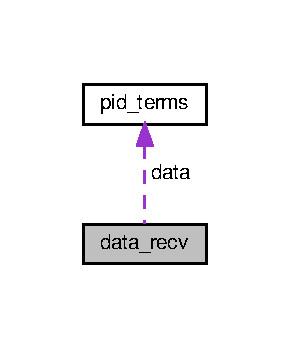
\includegraphics[width=139pt]{structdata__recv__coll__graph}
\end{center}
\end{figure}
\subsection*{Public Attributes}
\begin{DoxyCompactItemize}
\item 
struct \hyperlink{structpid__terms}{pid\+\_\+terms} \hyperlink{structdata__recv_af60b2e3d44df4ef57e1998ff55783920}{data}
\item 
esp\+\_\+err\+\_\+t \hyperlink{structdata__recv_a96d1938d8172e27035f655727f675273}{err}
\end{DoxyCompactItemize}


\subsection{Member Data Documentation}
\mbox{\Hypertarget{structdata__recv_af60b2e3d44df4ef57e1998ff55783920}\label{structdata__recv_af60b2e3d44df4ef57e1998ff55783920}} 
\index{data\+\_\+recv@{data\+\_\+recv}!data@{data}}
\index{data@{data}!data\+\_\+recv@{data\+\_\+recv}}
\subsubsection{\texorpdfstring{data}{data}}
{\footnotesize\ttfamily struct \hyperlink{structpid__terms}{pid\+\_\+terms} data\+\_\+recv\+::data}

\mbox{\Hypertarget{structdata__recv_a96d1938d8172e27035f655727f675273}\label{structdata__recv_a96d1938d8172e27035f655727f675273}} 
\index{data\+\_\+recv@{data\+\_\+recv}!err@{err}}
\index{err@{err}!data\+\_\+recv@{data\+\_\+recv}}
\subsubsection{\texorpdfstring{err}{err}}
{\footnotesize\ttfamily esp\+\_\+err\+\_\+t data\+\_\+recv\+::err}



The documentation for this struct was generated from the following file\+:\begin{DoxyCompactItemize}
\item 
/home/vedant/\+Programming/projects/pid-\/tuning-\/gui/esp\+\_\+codes/components/pid\+\_\+plotter/include/\hyperlink{transport_8h}{transport.\+h}\end{DoxyCompactItemize}

\hypertarget{structnetwork__data}{}\section{network\+\_\+data Struct Reference}
\label{structnetwork__data}\index{network\+\_\+data@{network\+\_\+data}}


{\ttfamily \#include $<$udp\+\_\+handler.\+h$>$}

\subsection*{Public Attributes}
\begin{DoxyCompactItemize}
\item 
char \hyperlink{structnetwork__data_a9346e7a82edd41c346d1528ef301469b}{rx\+\_\+buffer} \mbox{[}128\mbox{]}
\item 
char \hyperlink{structnetwork__data_a6e8bd28f3dda27bcedd8b6e39257bf9e}{addr\+\_\+str} \mbox{[}128\mbox{]}
\item 
int \hyperlink{structnetwork__data_a68f41514e366d2255d8ab802ec4ea146}{addr\+\_\+family}
\item 
int \hyperlink{structnetwork__data_a2e35f88440947101eeeb8dc91a43d5e5}{ip\+\_\+protocol}
\item 
struct sockaddr\+\_\+in \hyperlink{structnetwork__data_a553d72b8506e9098215451adffd330d4}{dest\+\_\+addr}
\item 
int \hyperlink{structnetwork__data_ab056807bd5bb97ce18f27e6b233de0b3}{sock}
\end{DoxyCompactItemize}


\subsection{Member Data Documentation}
\mbox{\Hypertarget{structnetwork__data_a68f41514e366d2255d8ab802ec4ea146}\label{structnetwork__data_a68f41514e366d2255d8ab802ec4ea146}} 
\index{network\+\_\+data@{network\+\_\+data}!addr\+\_\+family@{addr\+\_\+family}}
\index{addr\+\_\+family@{addr\+\_\+family}!network\+\_\+data@{network\+\_\+data}}
\subsubsection{\texorpdfstring{addr\+\_\+family}{addr\_family}}
{\footnotesize\ttfamily int network\+\_\+data\+::addr\+\_\+family}

\mbox{\Hypertarget{structnetwork__data_a6e8bd28f3dda27bcedd8b6e39257bf9e}\label{structnetwork__data_a6e8bd28f3dda27bcedd8b6e39257bf9e}} 
\index{network\+\_\+data@{network\+\_\+data}!addr\+\_\+str@{addr\+\_\+str}}
\index{addr\+\_\+str@{addr\+\_\+str}!network\+\_\+data@{network\+\_\+data}}
\subsubsection{\texorpdfstring{addr\+\_\+str}{addr\_str}}
{\footnotesize\ttfamily char network\+\_\+data\+::addr\+\_\+str\mbox{[}128\mbox{]}}

\mbox{\Hypertarget{structnetwork__data_a553d72b8506e9098215451adffd330d4}\label{structnetwork__data_a553d72b8506e9098215451adffd330d4}} 
\index{network\+\_\+data@{network\+\_\+data}!dest\+\_\+addr@{dest\+\_\+addr}}
\index{dest\+\_\+addr@{dest\+\_\+addr}!network\+\_\+data@{network\+\_\+data}}
\subsubsection{\texorpdfstring{dest\+\_\+addr}{dest\_addr}}
{\footnotesize\ttfamily struct sockaddr\+\_\+in network\+\_\+data\+::dest\+\_\+addr}

\mbox{\Hypertarget{structnetwork__data_a2e35f88440947101eeeb8dc91a43d5e5}\label{structnetwork__data_a2e35f88440947101eeeb8dc91a43d5e5}} 
\index{network\+\_\+data@{network\+\_\+data}!ip\+\_\+protocol@{ip\+\_\+protocol}}
\index{ip\+\_\+protocol@{ip\+\_\+protocol}!network\+\_\+data@{network\+\_\+data}}
\subsubsection{\texorpdfstring{ip\+\_\+protocol}{ip\_protocol}}
{\footnotesize\ttfamily int network\+\_\+data\+::ip\+\_\+protocol}

\mbox{\Hypertarget{structnetwork__data_a9346e7a82edd41c346d1528ef301469b}\label{structnetwork__data_a9346e7a82edd41c346d1528ef301469b}} 
\index{network\+\_\+data@{network\+\_\+data}!rx\+\_\+buffer@{rx\+\_\+buffer}}
\index{rx\+\_\+buffer@{rx\+\_\+buffer}!network\+\_\+data@{network\+\_\+data}}
\subsubsection{\texorpdfstring{rx\+\_\+buffer}{rx\_buffer}}
{\footnotesize\ttfamily char network\+\_\+data\+::rx\+\_\+buffer\mbox{[}128\mbox{]}}

\mbox{\Hypertarget{structnetwork__data_ab056807bd5bb97ce18f27e6b233de0b3}\label{structnetwork__data_ab056807bd5bb97ce18f27e6b233de0b3}} 
\index{network\+\_\+data@{network\+\_\+data}!sock@{sock}}
\index{sock@{sock}!network\+\_\+data@{network\+\_\+data}}
\subsubsection{\texorpdfstring{sock}{sock}}
{\footnotesize\ttfamily int network\+\_\+data\+::sock}



The documentation for this struct was generated from the following file\+:\begin{DoxyCompactItemize}
\item 
/home/vedant/\+Programming/projects/pid-\/tuning-\/gui/esp\+\_\+codes/components/pid\+\_\+plotter/include/\hyperlink{udp__handler_8h}{udp\+\_\+handler.\+h}\end{DoxyCompactItemize}

\hypertarget{structpid__const}{}\section{pid\+\_\+const Struct Reference}
\label{structpid__const}\index{pid\+\_\+const@{pid\+\_\+const}}


{\ttfamily \#include $<$json\+\_\+handler.\+h$>$}

\subsection*{Public Attributes}
\begin{DoxyCompactItemize}
\item 
float \hyperlink{structpid__const_a5ae3ec87567130989aa8dd833718c16a}{kp}
\item 
float \hyperlink{structpid__const_a29e400ad2fbe11cc68925c837956c1ab}{ki}
\item 
float \hyperlink{structpid__const_a5e6af6c51f63c03fe0fdf7705497e234}{kd}
\item 
float \hyperlink{structpid__const_a19b1118c03f705f3b693216e8f22d98a}{setpoint}
\end{DoxyCompactItemize}


\subsection{Member Data Documentation}
\mbox{\Hypertarget{structpid__const_a5e6af6c51f63c03fe0fdf7705497e234}\label{structpid__const_a5e6af6c51f63c03fe0fdf7705497e234}} 
\index{pid\+\_\+const@{pid\+\_\+const}!kd@{kd}}
\index{kd@{kd}!pid\+\_\+const@{pid\+\_\+const}}
\subsubsection{\texorpdfstring{kd}{kd}}
{\footnotesize\ttfamily float pid\+\_\+const\+::kd}

\mbox{\Hypertarget{structpid__const_a29e400ad2fbe11cc68925c837956c1ab}\label{structpid__const_a29e400ad2fbe11cc68925c837956c1ab}} 
\index{pid\+\_\+const@{pid\+\_\+const}!ki@{ki}}
\index{ki@{ki}!pid\+\_\+const@{pid\+\_\+const}}
\subsubsection{\texorpdfstring{ki}{ki}}
{\footnotesize\ttfamily float pid\+\_\+const\+::ki}

\mbox{\Hypertarget{structpid__const_a5ae3ec87567130989aa8dd833718c16a}\label{structpid__const_a5ae3ec87567130989aa8dd833718c16a}} 
\index{pid\+\_\+const@{pid\+\_\+const}!kp@{kp}}
\index{kp@{kp}!pid\+\_\+const@{pid\+\_\+const}}
\subsubsection{\texorpdfstring{kp}{kp}}
{\footnotesize\ttfamily float pid\+\_\+const\+::kp}

\mbox{\Hypertarget{structpid__const_a19b1118c03f705f3b693216e8f22d98a}\label{structpid__const_a19b1118c03f705f3b693216e8f22d98a}} 
\index{pid\+\_\+const@{pid\+\_\+const}!setpoint@{setpoint}}
\index{setpoint@{setpoint}!pid\+\_\+const@{pid\+\_\+const}}
\subsubsection{\texorpdfstring{setpoint}{setpoint}}
{\footnotesize\ttfamily float pid\+\_\+const\+::setpoint}



The documentation for this struct was generated from the following file\+:\begin{DoxyCompactItemize}
\item 
/home/vedant/\+Programming/projects/pid-\/tuning-\/gui/esp\+\_\+codes/components/pid\+\_\+plotter/include/\hyperlink{json__handler_8h}{json\+\_\+handler.\+h}\end{DoxyCompactItemize}

\hypertarget{structpid__terms}{}\section{pid\+\_\+terms Struct Reference}
\label{structpid__terms}\index{pid\+\_\+terms@{pid\+\_\+terms}}


{\ttfamily \#include $<$transport.\+h$>$}

\subsection*{Public Attributes}
\begin{DoxyCompactItemize}
\item 
float \hyperlink{structpid__terms_ab4c7f8712a43d4fe1b8932783f286c22}{current}
\item 
float \hyperlink{structpid__terms_a8073092d43a680432fa0f7784a7aef29}{error}
\item 
float \hyperlink{structpid__terms_af930983320efcf1d96d3b7cb85fee908}{P}
\item 
float \hyperlink{structpid__terms_af72ae69eaa9faeab7273dcbd847fdee9}{I}
\item 
float \hyperlink{structpid__terms_a864b7035292cd484f321d0f52a5a68d8}{D}
\end{DoxyCompactItemize}


\subsection{Member Data Documentation}
\mbox{\Hypertarget{structpid__terms_ab4c7f8712a43d4fe1b8932783f286c22}\label{structpid__terms_ab4c7f8712a43d4fe1b8932783f286c22}} 
\index{pid\+\_\+terms@{pid\+\_\+terms}!current@{current}}
\index{current@{current}!pid\+\_\+terms@{pid\+\_\+terms}}
\subsubsection{\texorpdfstring{current}{current}}
{\footnotesize\ttfamily float pid\+\_\+terms\+::current}

\mbox{\Hypertarget{structpid__terms_a864b7035292cd484f321d0f52a5a68d8}\label{structpid__terms_a864b7035292cd484f321d0f52a5a68d8}} 
\index{pid\+\_\+terms@{pid\+\_\+terms}!D@{D}}
\index{D@{D}!pid\+\_\+terms@{pid\+\_\+terms}}
\subsubsection{\texorpdfstring{D}{D}}
{\footnotesize\ttfamily float pid\+\_\+terms\+::D}

\mbox{\Hypertarget{structpid__terms_a8073092d43a680432fa0f7784a7aef29}\label{structpid__terms_a8073092d43a680432fa0f7784a7aef29}} 
\index{pid\+\_\+terms@{pid\+\_\+terms}!error@{error}}
\index{error@{error}!pid\+\_\+terms@{pid\+\_\+terms}}
\subsubsection{\texorpdfstring{error}{error}}
{\footnotesize\ttfamily float pid\+\_\+terms\+::error}

\mbox{\Hypertarget{structpid__terms_af72ae69eaa9faeab7273dcbd847fdee9}\label{structpid__terms_af72ae69eaa9faeab7273dcbd847fdee9}} 
\index{pid\+\_\+terms@{pid\+\_\+terms}!I@{I}}
\index{I@{I}!pid\+\_\+terms@{pid\+\_\+terms}}
\subsubsection{\texorpdfstring{I}{I}}
{\footnotesize\ttfamily float pid\+\_\+terms\+::I}

\mbox{\Hypertarget{structpid__terms_af930983320efcf1d96d3b7cb85fee908}\label{structpid__terms_af930983320efcf1d96d3b7cb85fee908}} 
\index{pid\+\_\+terms@{pid\+\_\+terms}!P@{P}}
\index{P@{P}!pid\+\_\+terms@{pid\+\_\+terms}}
\subsubsection{\texorpdfstring{P}{P}}
{\footnotesize\ttfamily float pid\+\_\+terms\+::P}



The documentation for this struct was generated from the following file\+:\begin{DoxyCompactItemize}
\item 
/home/vedant/\+Programming/projects/pid-\/tuning-\/gui/esp\+\_\+codes/components/pid\+\_\+plotter/include/\hyperlink{transport_8h}{transport.\+h}\end{DoxyCompactItemize}

\hypertarget{structtcp__network__data}{}\section{tcp\+\_\+network\+\_\+data Struct Reference}
\label{structtcp__network__data}\index{tcp\+\_\+network\+\_\+data@{tcp\+\_\+network\+\_\+data}}


{\ttfamily \#include $<$tcp\+\_\+handler.\+h$>$}

\subsection*{Public Attributes}
\begin{DoxyCompactItemize}
\item 
char \hyperlink{structtcp__network__data_aec4bca454d64124cd3a4b001f4a551cc}{rx\+\_\+buffer} \mbox{[}128\mbox{]}
\item 
char \hyperlink{structtcp__network__data_a5bb07a33391c99faa2caab2ef4477944}{addr\+\_\+str} \mbox{[}128\mbox{]}
\item 
int \hyperlink{structtcp__network__data_a901043d5d480118c9e8661464465ae95}{addr\+\_\+family}
\item 
int \hyperlink{structtcp__network__data_ac9025540ea4138efba1544b3fbbb2db3}{ip\+\_\+protocol}
\item 
struct sockaddr\+\_\+in \hyperlink{structtcp__network__data_aac1fae2cd9f342a287fc728c2171e3d1}{dest\+\_\+addr}
\item 
int \hyperlink{structtcp__network__data_a78063825cce60cb5f121e2c87ccb6dbb}{sock}
\end{DoxyCompactItemize}


\subsection{Member Data Documentation}
\mbox{\Hypertarget{structtcp__network__data_a901043d5d480118c9e8661464465ae95}\label{structtcp__network__data_a901043d5d480118c9e8661464465ae95}} 
\index{tcp\+\_\+network\+\_\+data@{tcp\+\_\+network\+\_\+data}!addr\+\_\+family@{addr\+\_\+family}}
\index{addr\+\_\+family@{addr\+\_\+family}!tcp\+\_\+network\+\_\+data@{tcp\+\_\+network\+\_\+data}}
\subsubsection{\texorpdfstring{addr\+\_\+family}{addr\_family}}
{\footnotesize\ttfamily int tcp\+\_\+network\+\_\+data\+::addr\+\_\+family}

\mbox{\Hypertarget{structtcp__network__data_a5bb07a33391c99faa2caab2ef4477944}\label{structtcp__network__data_a5bb07a33391c99faa2caab2ef4477944}} 
\index{tcp\+\_\+network\+\_\+data@{tcp\+\_\+network\+\_\+data}!addr\+\_\+str@{addr\+\_\+str}}
\index{addr\+\_\+str@{addr\+\_\+str}!tcp\+\_\+network\+\_\+data@{tcp\+\_\+network\+\_\+data}}
\subsubsection{\texorpdfstring{addr\+\_\+str}{addr\_str}}
{\footnotesize\ttfamily char tcp\+\_\+network\+\_\+data\+::addr\+\_\+str\mbox{[}128\mbox{]}}

\mbox{\Hypertarget{structtcp__network__data_aac1fae2cd9f342a287fc728c2171e3d1}\label{structtcp__network__data_aac1fae2cd9f342a287fc728c2171e3d1}} 
\index{tcp\+\_\+network\+\_\+data@{tcp\+\_\+network\+\_\+data}!dest\+\_\+addr@{dest\+\_\+addr}}
\index{dest\+\_\+addr@{dest\+\_\+addr}!tcp\+\_\+network\+\_\+data@{tcp\+\_\+network\+\_\+data}}
\subsubsection{\texorpdfstring{dest\+\_\+addr}{dest\_addr}}
{\footnotesize\ttfamily struct sockaddr\+\_\+in tcp\+\_\+network\+\_\+data\+::dest\+\_\+addr}

\mbox{\Hypertarget{structtcp__network__data_ac9025540ea4138efba1544b3fbbb2db3}\label{structtcp__network__data_ac9025540ea4138efba1544b3fbbb2db3}} 
\index{tcp\+\_\+network\+\_\+data@{tcp\+\_\+network\+\_\+data}!ip\+\_\+protocol@{ip\+\_\+protocol}}
\index{ip\+\_\+protocol@{ip\+\_\+protocol}!tcp\+\_\+network\+\_\+data@{tcp\+\_\+network\+\_\+data}}
\subsubsection{\texorpdfstring{ip\+\_\+protocol}{ip\_protocol}}
{\footnotesize\ttfamily int tcp\+\_\+network\+\_\+data\+::ip\+\_\+protocol}

\mbox{\Hypertarget{structtcp__network__data_aec4bca454d64124cd3a4b001f4a551cc}\label{structtcp__network__data_aec4bca454d64124cd3a4b001f4a551cc}} 
\index{tcp\+\_\+network\+\_\+data@{tcp\+\_\+network\+\_\+data}!rx\+\_\+buffer@{rx\+\_\+buffer}}
\index{rx\+\_\+buffer@{rx\+\_\+buffer}!tcp\+\_\+network\+\_\+data@{tcp\+\_\+network\+\_\+data}}
\subsubsection{\texorpdfstring{rx\+\_\+buffer}{rx\_buffer}}
{\footnotesize\ttfamily char tcp\+\_\+network\+\_\+data\+::rx\+\_\+buffer\mbox{[}128\mbox{]}}

\mbox{\Hypertarget{structtcp__network__data_a78063825cce60cb5f121e2c87ccb6dbb}\label{structtcp__network__data_a78063825cce60cb5f121e2c87ccb6dbb}} 
\index{tcp\+\_\+network\+\_\+data@{tcp\+\_\+network\+\_\+data}!sock@{sock}}
\index{sock@{sock}!tcp\+\_\+network\+\_\+data@{tcp\+\_\+network\+\_\+data}}
\subsubsection{\texorpdfstring{sock}{sock}}
{\footnotesize\ttfamily int tcp\+\_\+network\+\_\+data\+::sock}



The documentation for this struct was generated from the following file\+:\begin{DoxyCompactItemize}
\item 
/home/vedant/\+Programming/projects/pid-\/tuning-\/gui/esp\+\_\+codes/components/pid\+\_\+plotter/include/\hyperlink{tcp__handler_8h}{tcp\+\_\+handler.\+h}\end{DoxyCompactItemize}

\chapter{File Documentation}
\hypertarget{json__handler_8h}{}\section{/home/vedant/\+Programming/projects/pid-\/tuning-\/gui/esp\+\_\+codes/components/pid\+\_\+plotter/include/json\+\_\+handler.h File Reference}
\label{json__handler_8h}\index{/home/vedant/\+Programming/projects/pid-\/tuning-\/gui/esp\+\_\+codes/components/pid\+\_\+plotter/include/json\+\_\+handler.\+h@{/home/vedant/\+Programming/projects/pid-\/tuning-\/gui/esp\+\_\+codes/components/pid\+\_\+plotter/include/json\+\_\+handler.\+h}}
{\ttfamily \#include \char`\"{}c\+J\+S\+O\+N.\+h\char`\"{}}\newline
{\ttfamily \#include \char`\"{}stdio.\+h\char`\"{}}\newline
Include dependency graph for json\+\_\+handler.\+h\+:
\nopagebreak
\begin{figure}[H]
\begin{center}
\leavevmode
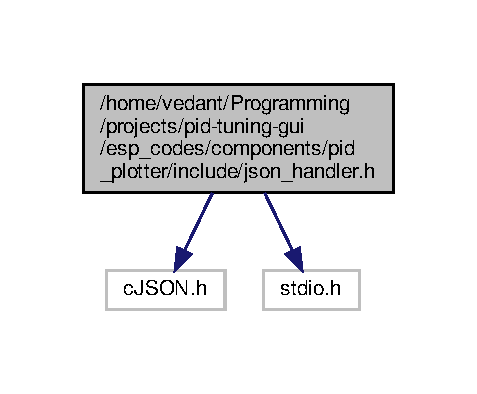
\includegraphics[width=229pt]{json__handler_8h__incl}
\end{center}
\end{figure}
This graph shows which files directly or indirectly include this file\+:
\nopagebreak
\begin{figure}[H]
\begin{center}
\leavevmode
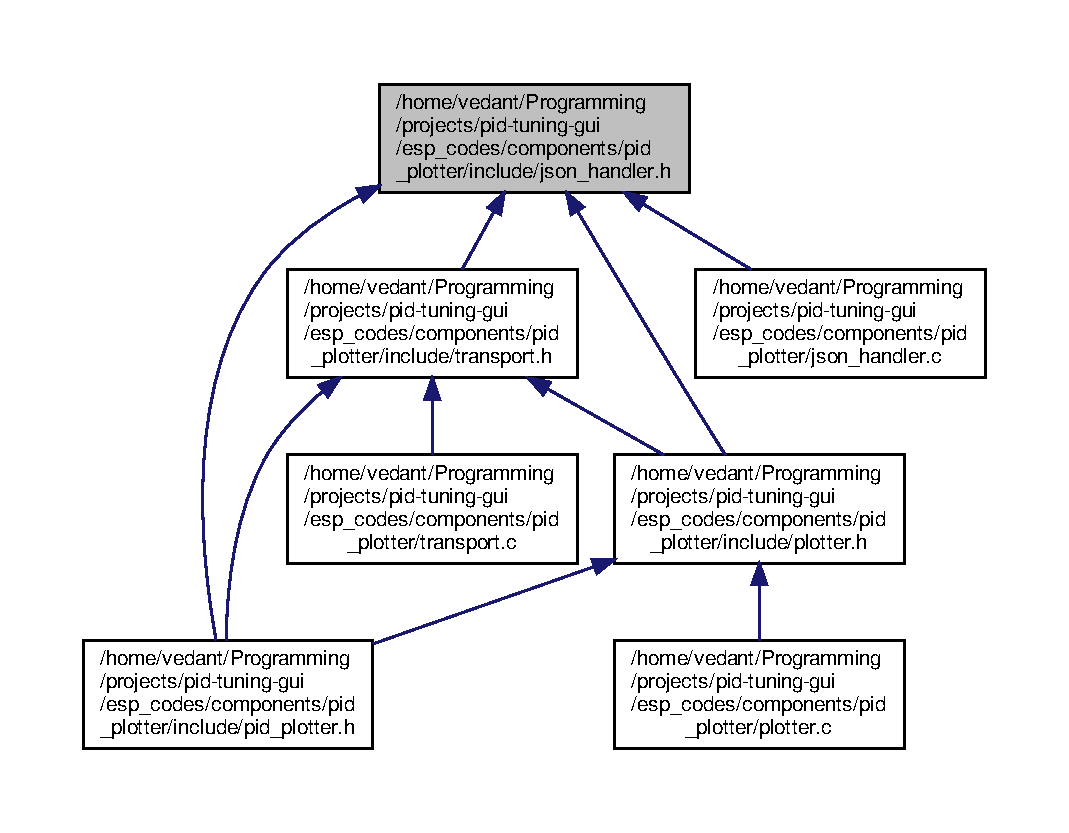
\includegraphics[width=350pt]{json__handler_8h__dep__incl}
\end{center}
\end{figure}
\subsection*{Classes}
\begin{DoxyCompactItemize}
\item 
struct \hyperlink{structpid__const}{pid\+\_\+const}
\end{DoxyCompactItemize}
\subsection*{Functions}
\begin{DoxyCompactItemize}
\item 
char $\ast$ \hyperlink{json__handler_8h_a229aa3d7fb017d31499a5e29b78b7f08}{create\+\_\+pid\+\_\+data\+\_\+to\+\_\+json} (float current, float error, float P, float I, float D)
\begin{DoxyCompactList}\small\item\em Converts P\+ID data to a json string. \end{DoxyCompactList}\item 
struct \hyperlink{structpid__const}{pid\+\_\+const} \hyperlink{json__handler_8h_a5a00fbe2cfe762fae40bd73932ddb072}{read\+\_\+pid\+\_\+data\+\_\+from\+\_\+json} (const char $\ast$data)
\begin{DoxyCompactList}\small\item\em Reads P\+ID constant data from a json formatted string. \end{DoxyCompactList}\end{DoxyCompactItemize}


\subsection{Function Documentation}
\mbox{\Hypertarget{json__handler_8h_a229aa3d7fb017d31499a5e29b78b7f08}\label{json__handler_8h_a229aa3d7fb017d31499a5e29b78b7f08}} 
\index{json\+\_\+handler.\+h@{json\+\_\+handler.\+h}!create\+\_\+pid\+\_\+data\+\_\+to\+\_\+json@{create\+\_\+pid\+\_\+data\+\_\+to\+\_\+json}}
\index{create\+\_\+pid\+\_\+data\+\_\+to\+\_\+json@{create\+\_\+pid\+\_\+data\+\_\+to\+\_\+json}!json\+\_\+handler.\+h@{json\+\_\+handler.\+h}}
\subsubsection{\texorpdfstring{create\+\_\+pid\+\_\+data\+\_\+to\+\_\+json()}{create\_pid\_data\_to\_json()}}
{\footnotesize\ttfamily char$\ast$ create\+\_\+pid\+\_\+data\+\_\+to\+\_\+json (\begin{DoxyParamCaption}\item[{float}]{current,  }\item[{float}]{error,  }\item[{float}]{P,  }\item[{float}]{I,  }\item[{float}]{D }\end{DoxyParamCaption})}



Converts P\+ID data to a json string. 


\begin{DoxyParams}{Parameters}
{\em current} & current value \\
\hline
{\em error} & error value, deviation of current from setpoint \\
\hline
{\em P} & Value of Proportional Gain (P) \\
\hline
{\em I} & Value of Integral Gain (I) \\
\hline
{\em D} & Value of Derivative Gain (D) \\
\hline
\end{DoxyParams}
\begin{DoxyReturn}{Returns}
char$\ast$ -\/ Json string of the data sent through parameters. 
\end{DoxyReturn}
\mbox{\Hypertarget{json__handler_8h_a5a00fbe2cfe762fae40bd73932ddb072}\label{json__handler_8h_a5a00fbe2cfe762fae40bd73932ddb072}} 
\index{json\+\_\+handler.\+h@{json\+\_\+handler.\+h}!read\+\_\+pid\+\_\+data\+\_\+from\+\_\+json@{read\+\_\+pid\+\_\+data\+\_\+from\+\_\+json}}
\index{read\+\_\+pid\+\_\+data\+\_\+from\+\_\+json@{read\+\_\+pid\+\_\+data\+\_\+from\+\_\+json}!json\+\_\+handler.\+h@{json\+\_\+handler.\+h}}
\subsubsection{\texorpdfstring{read\+\_\+pid\+\_\+data\+\_\+from\+\_\+json()}{read\_pid\_data\_from\_json()}}
{\footnotesize\ttfamily struct \hyperlink{structpid__const}{pid\+\_\+const} read\+\_\+pid\+\_\+data\+\_\+from\+\_\+json (\begin{DoxyParamCaption}\item[{const char $\ast$}]{data }\end{DoxyParamCaption})}



Reads P\+ID constant data from a json formatted string. 


\begin{DoxyParams}{Parameters}
{\em data} & Pointer to char array containging the json formatted string \\
\hline
\end{DoxyParams}
\begin{DoxyReturn}{Returns}
struct \hyperlink{structpid__const}{pid\+\_\+const} -\/ Returns a array of P\+ID constants, extracted from the json string 
\end{DoxyReturn}

\hypertarget{pid__plotter_8h}{}\section{/home/vedant/\+Programming/projects/pid-\/tuning-\/gui/esp\+\_\+codes/components/pid\+\_\+plotter/include/pid\+\_\+plotter.h File Reference}
\label{pid__plotter_8h}\index{/home/vedant/\+Programming/projects/pid-\/tuning-\/gui/esp\+\_\+codes/components/pid\+\_\+plotter/include/pid\+\_\+plotter.\+h@{/home/vedant/\+Programming/projects/pid-\/tuning-\/gui/esp\+\_\+codes/components/pid\+\_\+plotter/include/pid\+\_\+plotter.\+h}}
{\ttfamily \#include \char`\"{}json\+\_\+handler.\+h\char`\"{}}\newline
{\ttfamily \#include \char`\"{}udp\+\_\+handler.\+h\char`\"{}}\newline
{\ttfamily \#include \char`\"{}tcp\+\_\+handler.\+h\char`\"{}}\newline
{\ttfamily \#include \char`\"{}transport.\+h\char`\"{}}\newline
{\ttfamily \#include \char`\"{}plotter.\+h\char`\"{}}\newline
Include dependency graph for pid\+\_\+plotter.\+h\+:\nopagebreak
\begin{figure}[H]
\begin{center}
\leavevmode
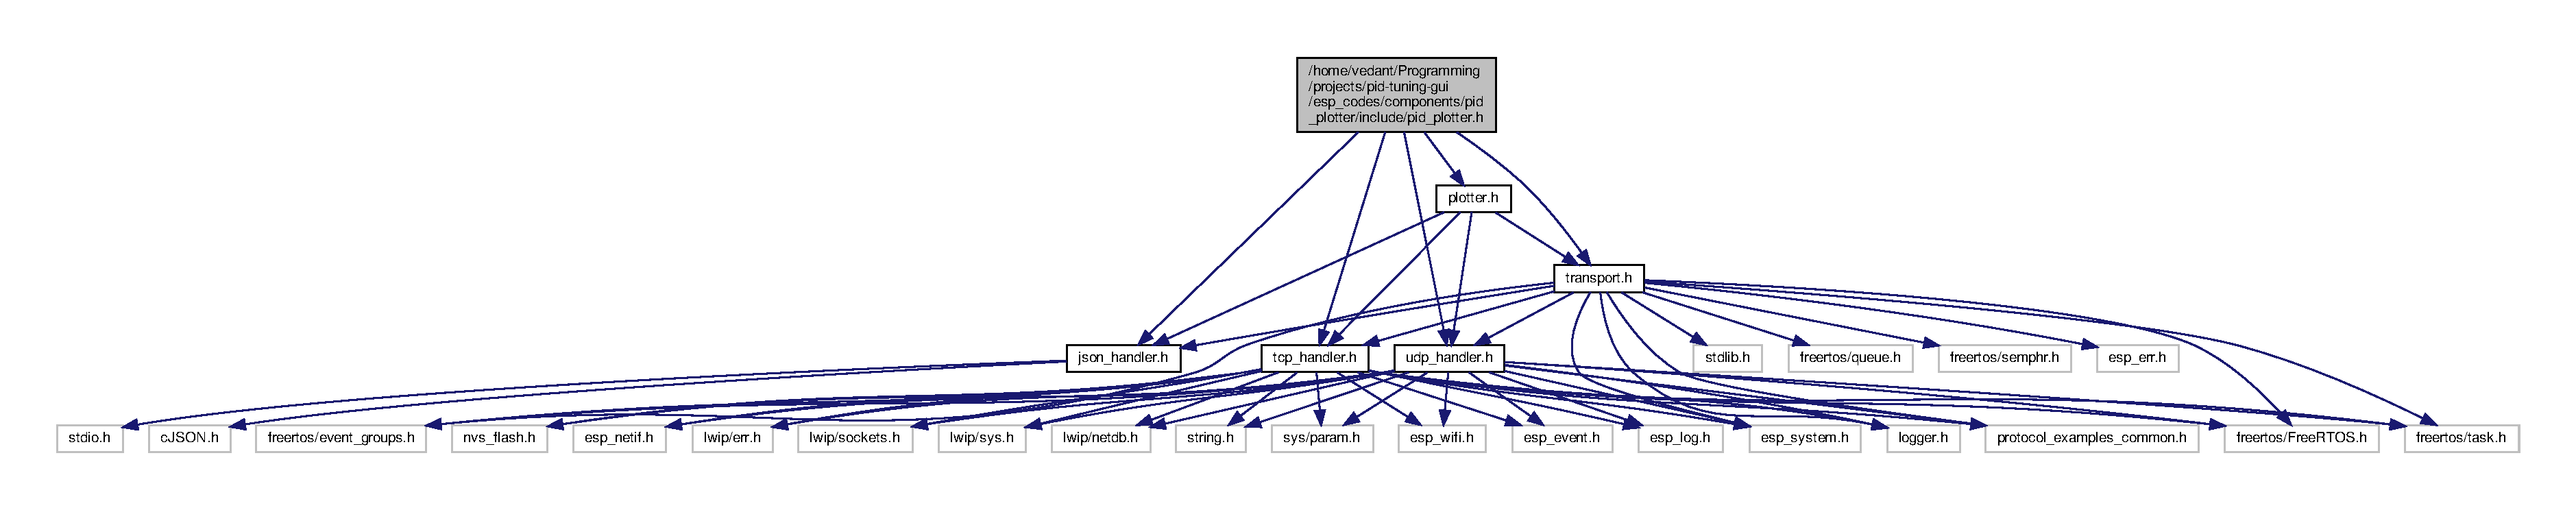
\includegraphics[width=350pt]{pid__plotter_8h__incl}
\end{center}
\end{figure}

\hypertarget{plotter_8h}{}\section{/home/vedant/\+Programming/projects/pid-\/tuning-\/gui/esp\+\_\+codes/components/pid\+\_\+plotter/include/plotter.h File Reference}
\label{plotter_8h}\index{/home/vedant/\+Programming/projects/pid-\/tuning-\/gui/esp\+\_\+codes/components/pid\+\_\+plotter/include/plotter.\+h@{/home/vedant/\+Programming/projects/pid-\/tuning-\/gui/esp\+\_\+codes/components/pid\+\_\+plotter/include/plotter.\+h}}
{\ttfamily \#include \char`\"{}json\+\_\+handler.\+h\char`\"{}}\newline
{\ttfamily \#include \char`\"{}udp\+\_\+handler.\+h\char`\"{}}\newline
{\ttfamily \#include \char`\"{}tcp\+\_\+handler.\+h\char`\"{}}\newline
{\ttfamily \#include \char`\"{}transport.\+h\char`\"{}}\newline
Include dependency graph for plotter.\+h\+:\nopagebreak
\begin{figure}[H]
\begin{center}
\leavevmode
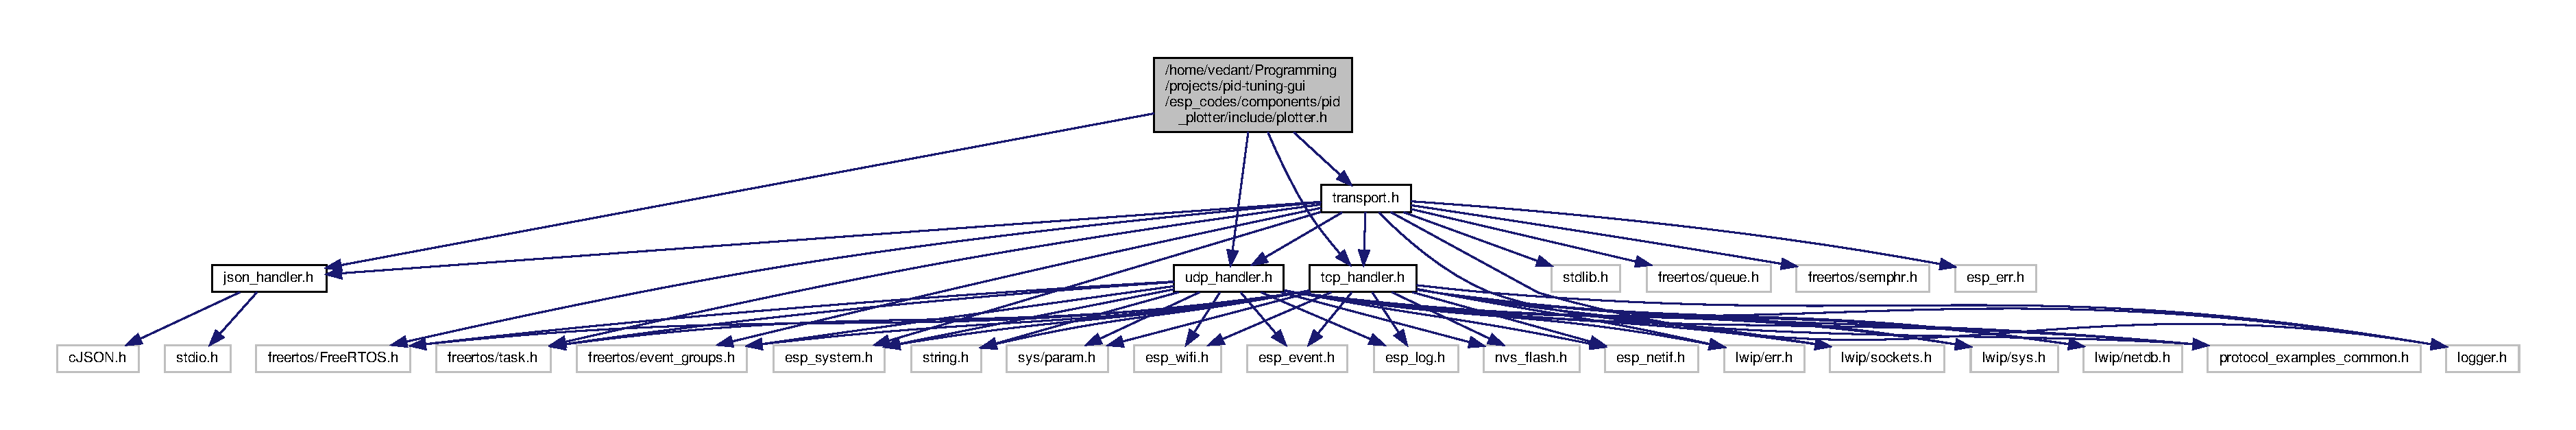
\includegraphics[width=350pt]{plotter_8h__incl}
\end{center}
\end{figure}
This graph shows which files directly or indirectly include this file\+:\nopagebreak
\begin{figure}[H]
\begin{center}
\leavevmode
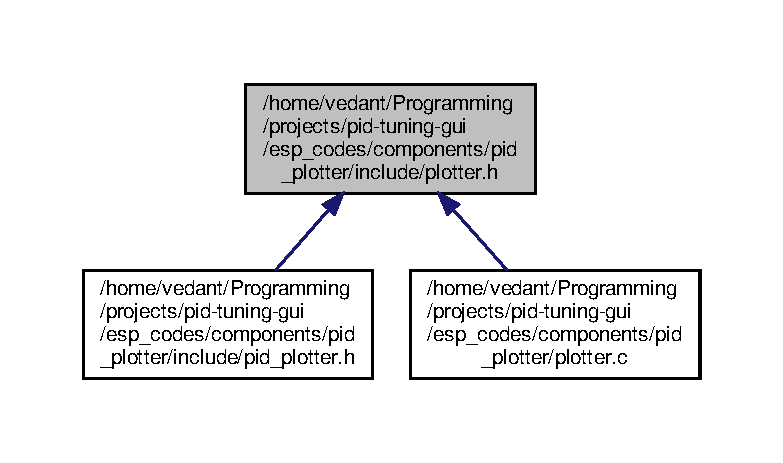
\includegraphics[width=350pt]{plotter_8h__dep__incl}
\end{center}
\end{figure}
\subsection*{Functions}
\begin{DoxyCompactItemize}
\item 
void \hyperlink{plotter_8h_acc8c0bc33035955e5c765b474fb33ef1}{plotter} ()
\begin{DoxyCompactList}\small\item\em Wrapper function to run the plotter functionality on a separate core. \end{DoxyCompactList}\end{DoxyCompactItemize}


\subsection{Function Documentation}
\mbox{\Hypertarget{plotter_8h_acc8c0bc33035955e5c765b474fb33ef1}\label{plotter_8h_acc8c0bc33035955e5c765b474fb33ef1}} 
\index{plotter.\+h@{plotter.\+h}!plotter@{plotter}}
\index{plotter@{plotter}!plotter.\+h@{plotter.\+h}}
\subsubsection{\texorpdfstring{plotter()}{plotter()}}
{\footnotesize\ttfamily void plotter (\begin{DoxyParamCaption}{ }\end{DoxyParamCaption})}



Wrapper function to run the plotter functionality on a separate core. 


\hypertarget{tcp__handler_8h}{}\section{/home/vedant/\+Programming/projects/pid-\/tuning-\/gui/esp\+\_\+codes/components/pid\+\_\+plotter/include/tcp\+\_\+handler.h File Reference}
\label{tcp__handler_8h}\index{/home/vedant/\+Programming/projects/pid-\/tuning-\/gui/esp\+\_\+codes/components/pid\+\_\+plotter/include/tcp\+\_\+handler.\+h@{/home/vedant/\+Programming/projects/pid-\/tuning-\/gui/esp\+\_\+codes/components/pid\+\_\+plotter/include/tcp\+\_\+handler.\+h}}
{\ttfamily \#include $<$string.\+h$>$}\newline
{\ttfamily \#include $<$sys/param.\+h$>$}\newline
{\ttfamily \#include \char`\"{}freertos/\+Free\+R\+T\+O\+S.\+h\char`\"{}}\newline
{\ttfamily \#include \char`\"{}freertos/task.\+h\char`\"{}}\newline
{\ttfamily \#include \char`\"{}freertos/event\+\_\+groups.\+h\char`\"{}}\newline
{\ttfamily \#include \char`\"{}esp\+\_\+system.\+h\char`\"{}}\newline
{\ttfamily \#include \char`\"{}esp\+\_\+wifi.\+h\char`\"{}}\newline
{\ttfamily \#include \char`\"{}esp\+\_\+event.\+h\char`\"{}}\newline
{\ttfamily \#include \char`\"{}esp\+\_\+log.\+h\char`\"{}}\newline
{\ttfamily \#include \char`\"{}nvs\+\_\+flash.\+h\char`\"{}}\newline
{\ttfamily \#include \char`\"{}esp\+\_\+netif.\+h\char`\"{}}\newline
{\ttfamily \#include \char`\"{}protocol\+\_\+examples\+\_\+common.\+h\char`\"{}}\newline
{\ttfamily \#include \char`\"{}logger.\+h\char`\"{}}\newline
{\ttfamily \#include \char`\"{}lwip/err.\+h\char`\"{}}\newline
{\ttfamily \#include \char`\"{}lwip/sockets.\+h\char`\"{}}\newline
{\ttfamily \#include \char`\"{}lwip/sys.\+h\char`\"{}}\newline
{\ttfamily \#include $<$lwip/netdb.\+h$>$}\newline
Include dependency graph for tcp\+\_\+handler.\+h\+:
\nopagebreak
\begin{figure}[H]
\begin{center}
\leavevmode
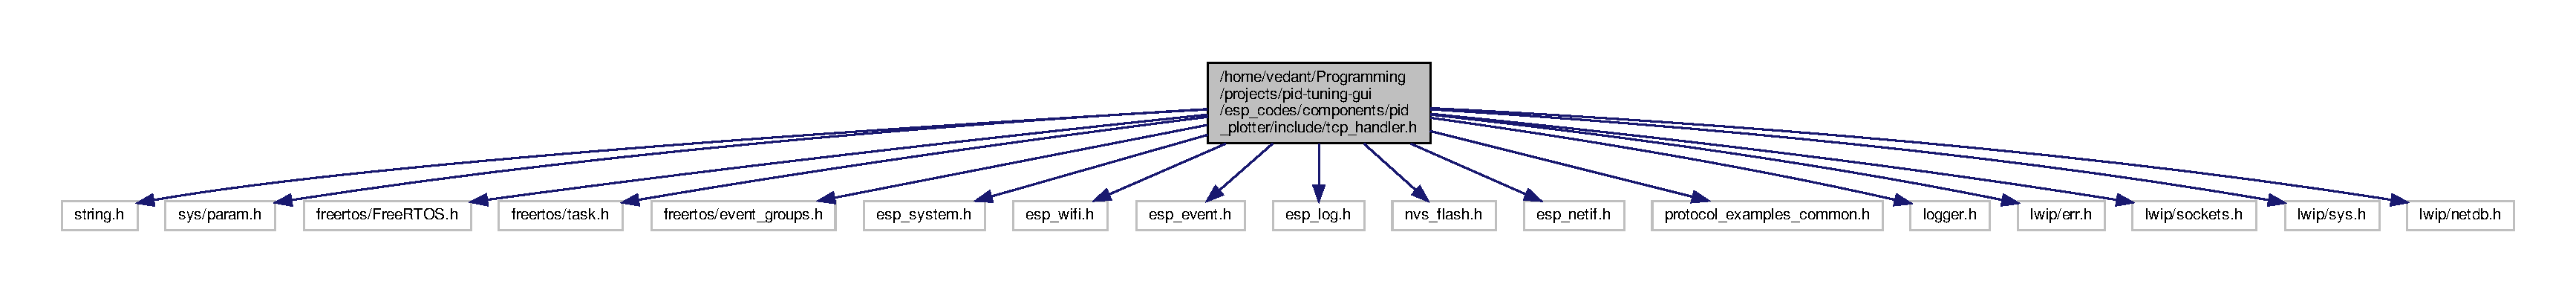
\includegraphics[width=350pt]{tcp__handler_8h__incl}
\end{center}
\end{figure}
This graph shows which files directly or indirectly include this file\+:
\nopagebreak
\begin{figure}[H]
\begin{center}
\leavevmode
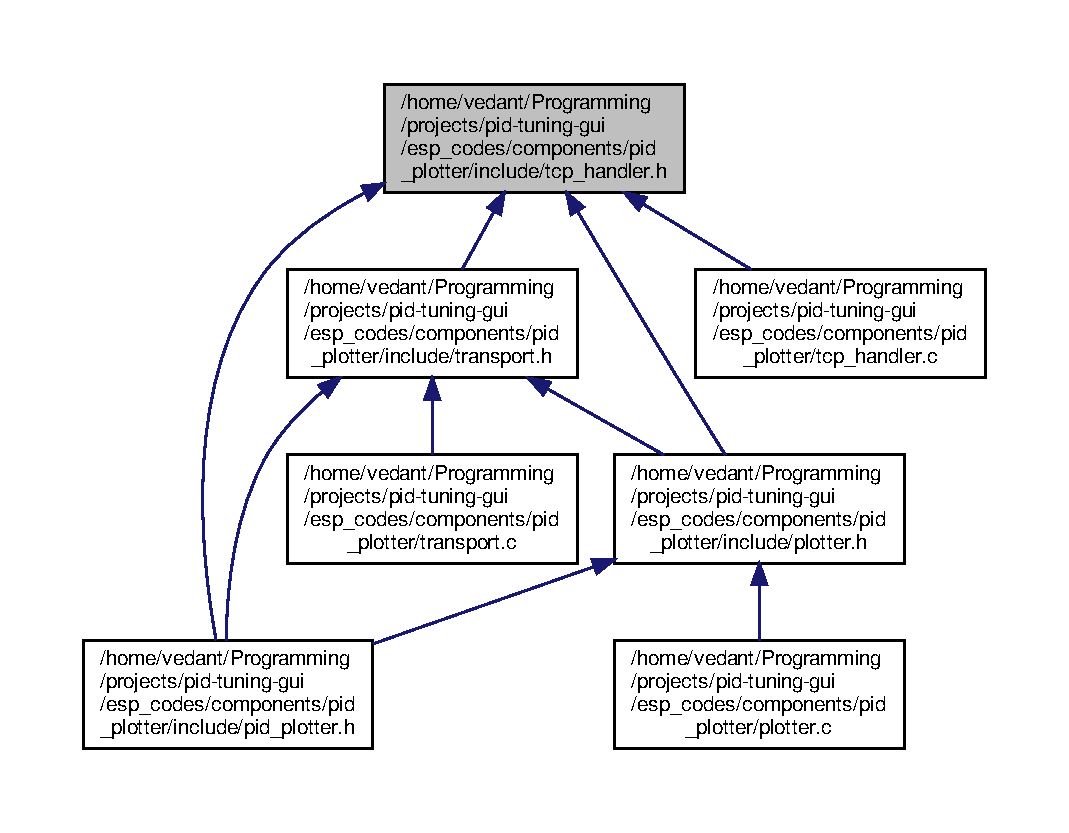
\includegraphics[width=350pt]{tcp__handler_8h__dep__incl}
\end{center}
\end{figure}
\subsection*{Classes}
\begin{DoxyCompactItemize}
\item 
struct \hyperlink{structtcp__network__data}{tcp\+\_\+network\+\_\+data}
\end{DoxyCompactItemize}
\subsection*{Macros}
\begin{DoxyCompactItemize}
\item 
\#define \hyperlink{tcp__handler_8h_a30e0c38ad4a5d0a16bfdd52ff64189b4}{T\+C\+P\+\_\+\+H\+O\+S\+T\+\_\+\+I\+P\+\_\+\+A\+D\+DR}~C\+O\+N\+F\+I\+G\+\_\+\+T\+C\+P\+\_\+\+I\+P\+\_\+\+A\+D\+D\+R\+E\+SS
\item 
\#define \hyperlink{tcp__handler_8h_a637b73f06ee87043251d022f87a8f3d4}{T\+C\+P\+\_\+\+P\+O\+RT}~C\+O\+N\+F\+I\+G\+\_\+\+T\+C\+P\+\_\+\+P\+O\+RT
\end{DoxyCompactItemize}
\subsection*{Functions}
\begin{DoxyCompactItemize}
\item 
void \hyperlink{tcp__handler_8h_a6be7633691ba5c012155871a84ade82e}{tcp\+\_\+network\+\_\+manager} (struct \hyperlink{structtcp__network__data}{tcp\+\_\+network\+\_\+data} $\ast$nm)
\begin{DoxyCompactList}\small\item\em Manages T\+CP connection to the server. \end{DoxyCompactList}\item 
int \hyperlink{tcp__handler_8h_a0ca62b309e39660b29ee7605b099ee54}{tcp\+\_\+send\+\_\+data} (struct \hyperlink{structtcp__network__data}{tcp\+\_\+network\+\_\+data} $\ast$nm, char $\ast$payload)
\begin{DoxyCompactList}\small\item\em Sends data to the server through a T\+CP socket. \end{DoxyCompactList}\item 
char $\ast$ \hyperlink{tcp__handler_8h_ae58555e8930155fcea5b1d16915db87b}{tcp\+\_\+recieve\+\_\+data} (struct \hyperlink{structtcp__network__data}{tcp\+\_\+network\+\_\+data} $\ast$nm)
\begin{DoxyCompactList}\small\item\em Receives data from T\+CP server. \end{DoxyCompactList}\item 
void \hyperlink{tcp__handler_8h_a6d6a248c21ebfece9f52fa7b580fabb5}{tcp\+\_\+close\+\_\+network\+\_\+manager} (struct \hyperlink{structtcp__network__data}{tcp\+\_\+network\+\_\+data} $\ast$nm)
\begin{DoxyCompactList}\small\item\em Shutdown active connection, deallocate memory. \end{DoxyCompactList}\end{DoxyCompactItemize}


\subsection{Macro Definition Documentation}
\mbox{\Hypertarget{tcp__handler_8h_a30e0c38ad4a5d0a16bfdd52ff64189b4}\label{tcp__handler_8h_a30e0c38ad4a5d0a16bfdd52ff64189b4}} 
\index{tcp\+\_\+handler.\+h@{tcp\+\_\+handler.\+h}!T\+C\+P\+\_\+\+H\+O\+S\+T\+\_\+\+I\+P\+\_\+\+A\+D\+DR@{T\+C\+P\+\_\+\+H\+O\+S\+T\+\_\+\+I\+P\+\_\+\+A\+D\+DR}}
\index{T\+C\+P\+\_\+\+H\+O\+S\+T\+\_\+\+I\+P\+\_\+\+A\+D\+DR@{T\+C\+P\+\_\+\+H\+O\+S\+T\+\_\+\+I\+P\+\_\+\+A\+D\+DR}!tcp\+\_\+handler.\+h@{tcp\+\_\+handler.\+h}}
\subsubsection{\texorpdfstring{T\+C\+P\+\_\+\+H\+O\+S\+T\+\_\+\+I\+P\+\_\+\+A\+D\+DR}{TCP\_HOST\_IP\_ADDR}}
{\footnotesize\ttfamily \#define T\+C\+P\+\_\+\+H\+O\+S\+T\+\_\+\+I\+P\+\_\+\+A\+D\+DR~C\+O\+N\+F\+I\+G\+\_\+\+T\+C\+P\+\_\+\+I\+P\+\_\+\+A\+D\+D\+R\+E\+SS}

\mbox{\Hypertarget{tcp__handler_8h_a637b73f06ee87043251d022f87a8f3d4}\label{tcp__handler_8h_a637b73f06ee87043251d022f87a8f3d4}} 
\index{tcp\+\_\+handler.\+h@{tcp\+\_\+handler.\+h}!T\+C\+P\+\_\+\+P\+O\+RT@{T\+C\+P\+\_\+\+P\+O\+RT}}
\index{T\+C\+P\+\_\+\+P\+O\+RT@{T\+C\+P\+\_\+\+P\+O\+RT}!tcp\+\_\+handler.\+h@{tcp\+\_\+handler.\+h}}
\subsubsection{\texorpdfstring{T\+C\+P\+\_\+\+P\+O\+RT}{TCP\_PORT}}
{\footnotesize\ttfamily \#define T\+C\+P\+\_\+\+P\+O\+RT~C\+O\+N\+F\+I\+G\+\_\+\+T\+C\+P\+\_\+\+P\+O\+RT}



\subsection{Function Documentation}
\mbox{\Hypertarget{tcp__handler_8h_a6d6a248c21ebfece9f52fa7b580fabb5}\label{tcp__handler_8h_a6d6a248c21ebfece9f52fa7b580fabb5}} 
\index{tcp\+\_\+handler.\+h@{tcp\+\_\+handler.\+h}!tcp\+\_\+close\+\_\+network\+\_\+manager@{tcp\+\_\+close\+\_\+network\+\_\+manager}}
\index{tcp\+\_\+close\+\_\+network\+\_\+manager@{tcp\+\_\+close\+\_\+network\+\_\+manager}!tcp\+\_\+handler.\+h@{tcp\+\_\+handler.\+h}}
\subsubsection{\texorpdfstring{tcp\+\_\+close\+\_\+network\+\_\+manager()}{tcp\_close\_network\_manager()}}
{\footnotesize\ttfamily void tcp\+\_\+close\+\_\+network\+\_\+manager (\begin{DoxyParamCaption}\item[{struct \hyperlink{structtcp__network__data}{tcp\+\_\+network\+\_\+data} $\ast$}]{nm }\end{DoxyParamCaption})}



Shutdown active connection, deallocate memory. 


\begin{DoxyParams}{Parameters}
{\em nm} & \hyperlink{structtcp__network__data}{tcp\+\_\+network\+\_\+data} struct which contains connection info \\
\hline
\end{DoxyParams}
\begin{DoxyReturn}{Returns}
void 
\end{DoxyReturn}
\mbox{\Hypertarget{tcp__handler_8h_a6be7633691ba5c012155871a84ade82e}\label{tcp__handler_8h_a6be7633691ba5c012155871a84ade82e}} 
\index{tcp\+\_\+handler.\+h@{tcp\+\_\+handler.\+h}!tcp\+\_\+network\+\_\+manager@{tcp\+\_\+network\+\_\+manager}}
\index{tcp\+\_\+network\+\_\+manager@{tcp\+\_\+network\+\_\+manager}!tcp\+\_\+handler.\+h@{tcp\+\_\+handler.\+h}}
\subsubsection{\texorpdfstring{tcp\+\_\+network\+\_\+manager()}{tcp\_network\_manager()}}
{\footnotesize\ttfamily void tcp\+\_\+network\+\_\+manager (\begin{DoxyParamCaption}\item[{struct \hyperlink{structtcp__network__data}{tcp\+\_\+network\+\_\+data} $\ast$}]{nm }\end{DoxyParamCaption})}



Manages T\+CP connection to the server. 


\begin{DoxyParams}{Parameters}
{\em nm} & \hyperlink{structtcp__network__data}{tcp\+\_\+network\+\_\+data} struct which contains necessary data for a T\+CP connection \\
\hline
\end{DoxyParams}
\begin{DoxyReturn}{Returns}
void 
\end{DoxyReturn}
\mbox{\Hypertarget{tcp__handler_8h_ae58555e8930155fcea5b1d16915db87b}\label{tcp__handler_8h_ae58555e8930155fcea5b1d16915db87b}} 
\index{tcp\+\_\+handler.\+h@{tcp\+\_\+handler.\+h}!tcp\+\_\+recieve\+\_\+data@{tcp\+\_\+recieve\+\_\+data}}
\index{tcp\+\_\+recieve\+\_\+data@{tcp\+\_\+recieve\+\_\+data}!tcp\+\_\+handler.\+h@{tcp\+\_\+handler.\+h}}
\subsubsection{\texorpdfstring{tcp\+\_\+recieve\+\_\+data()}{tcp\_recieve\_data()}}
{\footnotesize\ttfamily char$\ast$ tcp\+\_\+recieve\+\_\+data (\begin{DoxyParamCaption}\item[{struct \hyperlink{structtcp__network__data}{tcp\+\_\+network\+\_\+data} $\ast$}]{nm }\end{DoxyParamCaption})}



Receives data from T\+CP server. 


\begin{DoxyParams}{Parameters}
{\em nm} & \hyperlink{structtcp__network__data}{tcp\+\_\+network\+\_\+data} struct which contains connection info \\
\hline
\end{DoxyParams}
\begin{DoxyReturn}{Returns}
char array which contains data received 
\end{DoxyReturn}
\mbox{\Hypertarget{tcp__handler_8h_a0ca62b309e39660b29ee7605b099ee54}\label{tcp__handler_8h_a0ca62b309e39660b29ee7605b099ee54}} 
\index{tcp\+\_\+handler.\+h@{tcp\+\_\+handler.\+h}!tcp\+\_\+send\+\_\+data@{tcp\+\_\+send\+\_\+data}}
\index{tcp\+\_\+send\+\_\+data@{tcp\+\_\+send\+\_\+data}!tcp\+\_\+handler.\+h@{tcp\+\_\+handler.\+h}}
\subsubsection{\texorpdfstring{tcp\+\_\+send\+\_\+data()}{tcp\_send\_data()}}
{\footnotesize\ttfamily int tcp\+\_\+send\+\_\+data (\begin{DoxyParamCaption}\item[{struct \hyperlink{structtcp__network__data}{tcp\+\_\+network\+\_\+data} $\ast$}]{nm,  }\item[{char $\ast$}]{payload }\end{DoxyParamCaption})}



Sends data to the server through a T\+CP socket. 


\begin{DoxyParams}{Parameters}
{\em nm} & A pointer to \hyperlink{structtcp__network__data}{tcp\+\_\+network\+\_\+data} struct \\
\hline
{\em payload} & char array which contains data to be sent \\
\hline
\end{DoxyParams}
\begin{DoxyReturn}{Returns}
int -\/ returns -\/1 if sending failed, number of bytes sent if successfully sent the data 
\end{DoxyReturn}

\hypertarget{transport_8h}{}\section{/home/vedant/\+Programming/projects/pid-\/tuning-\/gui/esp\+\_\+codes/components/pid\+\_\+plotter/include/transport.h File Reference}
\label{transport_8h}\index{/home/vedant/\+Programming/projects/pid-\/tuning-\/gui/esp\+\_\+codes/components/pid\+\_\+plotter/include/transport.\+h@{/home/vedant/\+Programming/projects/pid-\/tuning-\/gui/esp\+\_\+codes/components/pid\+\_\+plotter/include/transport.\+h}}
{\ttfamily \#include $<$stdlib.\+h$>$}\newline
{\ttfamily \#include \char`\"{}udp\+\_\+handler.\+h\char`\"{}}\newline
{\ttfamily \#include \char`\"{}json\+\_\+handler.\+h\char`\"{}}\newline
{\ttfamily \#include \char`\"{}tcp\+\_\+handler.\+h\char`\"{}}\newline
{\ttfamily \#include \char`\"{}logger.\+h\char`\"{}}\newline
{\ttfamily \#include \char`\"{}freertos/\+Free\+R\+T\+O\+S.\+h\char`\"{}}\newline
{\ttfamily \#include \char`\"{}freertos/task.\+h\char`\"{}}\newline
{\ttfamily \#include \char`\"{}esp\+\_\+system.\+h\char`\"{}}\newline
{\ttfamily \#include \char`\"{}freertos/queue.\+h\char`\"{}}\newline
{\ttfamily \#include \char`\"{}freertos/event\+\_\+groups.\+h\char`\"{}}\newline
{\ttfamily \#include \char`\"{}freertos/semphr.\+h\char`\"{}}\newline
{\ttfamily \#include \char`\"{}esp\+\_\+err.\+h\char`\"{}}\newline
{\ttfamily \#include \char`\"{}protocol\+\_\+examples\+\_\+common.\+h\char`\"{}}\newline
Include dependency graph for transport.\+h\+:\nopagebreak
\begin{figure}[H]
\begin{center}
\leavevmode
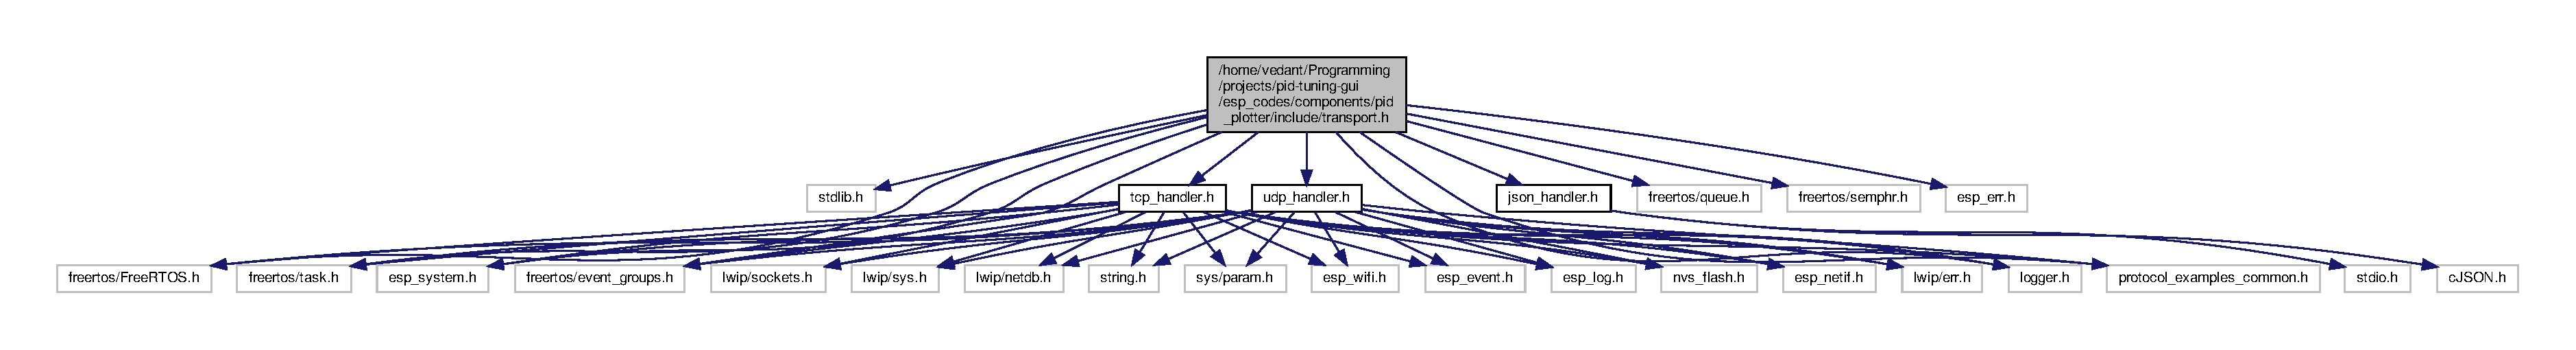
\includegraphics[width=350pt]{transport_8h__incl}
\end{center}
\end{figure}
This graph shows which files directly or indirectly include this file\+:\nopagebreak
\begin{figure}[H]
\begin{center}
\leavevmode
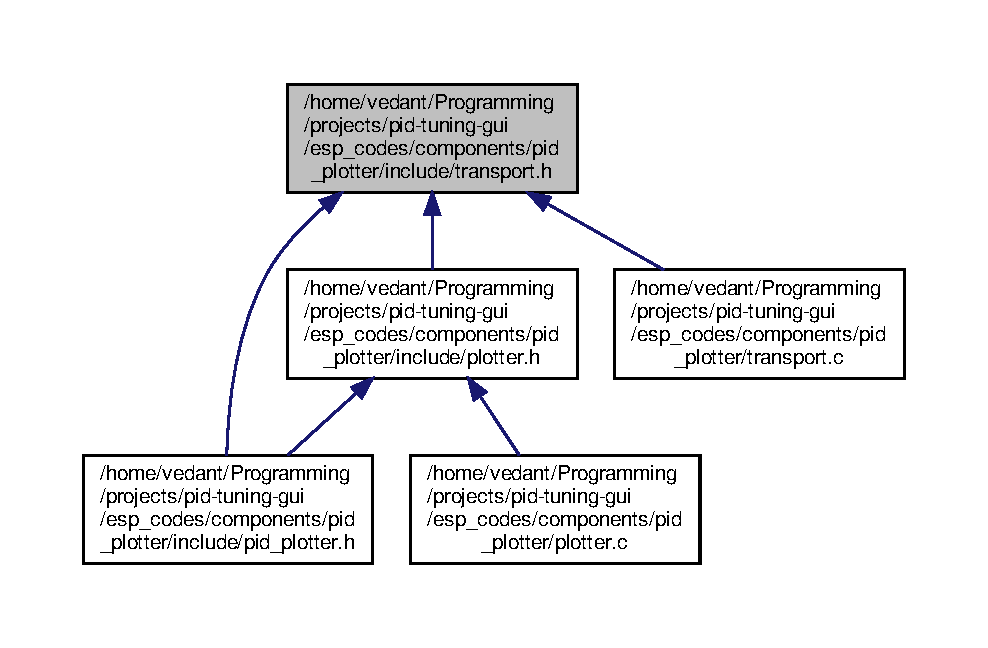
\includegraphics[width=350pt]{transport_8h__dep__incl}
\end{center}
\end{figure}
\subsection*{Classes}
\begin{DoxyCompactItemize}
\item 
struct \hyperlink{structpid__terms}{pid\+\_\+terms}
\item 
struct \hyperlink{structdata__recv}{data\+\_\+recv}
\end{DoxyCompactItemize}
\subsection*{Macros}
\begin{DoxyCompactItemize}
\item 
\#define \hyperlink{transport_8h_a81a6fc89c7bc286cb7360b155b1901bf}{M\+E\+S\+S\+A\+G\+E\+\_\+\+Q\+U\+E\+U\+E\+\_\+\+S\+I\+ZE}~C\+O\+N\+F\+I\+G\+\_\+\+M\+E\+S\+S\+A\+G\+E\+\_\+\+Q\+U\+E\+U\+E\+\_\+\+S\+I\+ZE
\end{DoxyCompactItemize}
\subsection*{Functions}
\begin{DoxyCompactItemize}
\item 
esp\+\_\+err\+\_\+t \hyperlink{transport_8h_a320afeaba56579760e7e3185a3d1fa02}{init\+\_\+queue} (void)
\begin{DoxyCompactList}\small\item\em Initialises message queue. \end{DoxyCompactList}\item 
void \hyperlink{transport_8h_a6afdab1f1ab02c6ed620949a7d32ffa4}{init\+\_\+transport} (void)
\begin{DoxyCompactList}\small\item\em Initialises transport, i.\+e. connect to wifi. \end{DoxyCompactList}\item 
esp\+\_\+err\+\_\+t \hyperlink{transport_8h_a3d23daa4cae5ba60d838c8a2b785462e}{send\+\_\+to\+\_\+queue} (struct \hyperlink{structpid__terms}{pid\+\_\+terms} pid\+\_\+data)
\begin{DoxyCompactList}\small\item\em Sends pid\+\_\+data struct to message queue. \end{DoxyCompactList}\item 
struct \hyperlink{structdata__recv}{data\+\_\+recv} \hyperlink{transport_8h_a3f717da7b4c254e710bbfd76625b15e4}{receive\+\_\+from\+\_\+queue} (void)
\begin{DoxyCompactList}\small\item\em Receive data from queue. \end{DoxyCompactList}\item 
void \hyperlink{transport_8h_a56e72500cb37fcbc087c3c3125ab7f8e}{pid\+\_\+transport} ()
\begin{DoxyCompactList}\small\item\em Handles U\+DP client, which sends \hyperlink{structpid__terms}{pid\+\_\+terms} received through message queue. \end{DoxyCompactList}\item 
void \hyperlink{transport_8h_acaba133d8c5e0cbadc4cfff68feca9fc}{pid\+\_\+const\+\_\+transport} ()
\begin{DoxyCompactList}\small\item\em Handles T\+CP client, which receives pid\+\_\+constants from server, and parses the data and stores it in a global struct pid\+\_\+const\+\_\+data. \end{DoxyCompactList}\item 
struct \hyperlink{structpid__const}{pid\+\_\+const} \hyperlink{transport_8h_aa37b5765ca807a54890c516c916e7e9b}{pid\+\_\+const\+\_\+read} ()
\begin{DoxyCompactList}\small\item\em Returns pid\+\_\+const\+\_\+data struct. Checks if the resource is blocked by mutex for writing or it is accessible, waits till pid\+\_\+const\+\_\+data is accessible and returns it. \end{DoxyCompactList}\end{DoxyCompactItemize}
\subsection*{Variables}
\begin{DoxyCompactItemize}
\item 
Task\+Handle\+\_\+t \hyperlink{transport_8h_afd5531c3e8b14bff72ce2bb5d9e37afb}{pid\+\_\+transport\+\_\+handle}
\item 
Task\+Handle\+\_\+t \hyperlink{transport_8h_af69ee3a89d006744edbe8e3039c6210d}{pid\+\_\+const\+\_\+transport\+\_\+handle}
\item 
Queue\+Handle\+\_\+t \hyperlink{transport_8h_a3b6a15c259cc8b4aff104b1ace175fc9}{pid\+\_\+struct\+\_\+queue}
\item 
Semaphore\+Handle\+\_\+t \hyperlink{transport_8h_a4e23be7e0ba011a32f7896896aaf186e}{pid\+\_\+const\+\_\+read\+\_\+write\+\_\+mutex}
\item 
struct \hyperlink{structpid__const}{pid\+\_\+const} \hyperlink{transport_8h_a73103b87c83e2ad74f75c8e400f58376}{pid\+\_\+const\+\_\+data}
\end{DoxyCompactItemize}


\subsection{Macro Definition Documentation}
\mbox{\Hypertarget{transport_8h_a81a6fc89c7bc286cb7360b155b1901bf}\label{transport_8h_a81a6fc89c7bc286cb7360b155b1901bf}} 
\index{transport.\+h@{transport.\+h}!M\+E\+S\+S\+A\+G\+E\+\_\+\+Q\+U\+E\+U\+E\+\_\+\+S\+I\+ZE@{M\+E\+S\+S\+A\+G\+E\+\_\+\+Q\+U\+E\+U\+E\+\_\+\+S\+I\+ZE}}
\index{M\+E\+S\+S\+A\+G\+E\+\_\+\+Q\+U\+E\+U\+E\+\_\+\+S\+I\+ZE@{M\+E\+S\+S\+A\+G\+E\+\_\+\+Q\+U\+E\+U\+E\+\_\+\+S\+I\+ZE}!transport.\+h@{transport.\+h}}
\subsubsection{\texorpdfstring{M\+E\+S\+S\+A\+G\+E\+\_\+\+Q\+U\+E\+U\+E\+\_\+\+S\+I\+ZE}{MESSAGE\_QUEUE\_SIZE}}
{\footnotesize\ttfamily \#define M\+E\+S\+S\+A\+G\+E\+\_\+\+Q\+U\+E\+U\+E\+\_\+\+S\+I\+ZE~C\+O\+N\+F\+I\+G\+\_\+\+M\+E\+S\+S\+A\+G\+E\+\_\+\+Q\+U\+E\+U\+E\+\_\+\+S\+I\+ZE}



\subsection{Function Documentation}
\mbox{\Hypertarget{transport_8h_a320afeaba56579760e7e3185a3d1fa02}\label{transport_8h_a320afeaba56579760e7e3185a3d1fa02}} 
\index{transport.\+h@{transport.\+h}!init\+\_\+queue@{init\+\_\+queue}}
\index{init\+\_\+queue@{init\+\_\+queue}!transport.\+h@{transport.\+h}}
\subsubsection{\texorpdfstring{init\+\_\+queue()}{init\_queue()}}
{\footnotesize\ttfamily esp\+\_\+err\+\_\+t init\+\_\+queue (\begin{DoxyParamCaption}\item[{void}]{ }\end{DoxyParamCaption})}



Initialises message queue. 

\begin{DoxyReturn}{Returns}
esp\+\_\+err\+\_\+t E\+S\+P\+\_\+\+OK -\/ if queue init sucessfully, E\+S\+P\+\_\+\+F\+A\+IL -\/ if queue init failed 
\end{DoxyReturn}
\mbox{\Hypertarget{transport_8h_a6afdab1f1ab02c6ed620949a7d32ffa4}\label{transport_8h_a6afdab1f1ab02c6ed620949a7d32ffa4}} 
\index{transport.\+h@{transport.\+h}!init\+\_\+transport@{init\+\_\+transport}}
\index{init\+\_\+transport@{init\+\_\+transport}!transport.\+h@{transport.\+h}}
\subsubsection{\texorpdfstring{init\+\_\+transport()}{init\_transport()}}
{\footnotesize\ttfamily void init\+\_\+transport (\begin{DoxyParamCaption}\item[{void}]{ }\end{DoxyParamCaption})}



Initialises transport, i.\+e. connect to wifi. 

\mbox{\Hypertarget{transport_8h_aa37b5765ca807a54890c516c916e7e9b}\label{transport_8h_aa37b5765ca807a54890c516c916e7e9b}} 
\index{transport.\+h@{transport.\+h}!pid\+\_\+const\+\_\+read@{pid\+\_\+const\+\_\+read}}
\index{pid\+\_\+const\+\_\+read@{pid\+\_\+const\+\_\+read}!transport.\+h@{transport.\+h}}
\subsubsection{\texorpdfstring{pid\+\_\+const\+\_\+read()}{pid\_const\_read()}}
{\footnotesize\ttfamily struct \hyperlink{structpid__const}{pid\+\_\+const} pid\+\_\+const\+\_\+read (\begin{DoxyParamCaption}{ }\end{DoxyParamCaption})}



Returns pid\+\_\+const\+\_\+data struct. Checks if the resource is blocked by mutex for writing or it is accessible, waits till pid\+\_\+const\+\_\+data is accessible and returns it. 

\begin{DoxyReturn}{Returns}
struct \hyperlink{structpid__const}{pid\+\_\+const} -\/ Returns pid\+\_\+const\+\_\+data, can be used to access Kp, Ki, Kd and current values 
\end{DoxyReturn}
\mbox{\Hypertarget{transport_8h_acaba133d8c5e0cbadc4cfff68feca9fc}\label{transport_8h_acaba133d8c5e0cbadc4cfff68feca9fc}} 
\index{transport.\+h@{transport.\+h}!pid\+\_\+const\+\_\+transport@{pid\+\_\+const\+\_\+transport}}
\index{pid\+\_\+const\+\_\+transport@{pid\+\_\+const\+\_\+transport}!transport.\+h@{transport.\+h}}
\subsubsection{\texorpdfstring{pid\+\_\+const\+\_\+transport()}{pid\_const\_transport()}}
{\footnotesize\ttfamily void pid\+\_\+const\+\_\+transport (\begin{DoxyParamCaption}{ }\end{DoxyParamCaption})}



Handles T\+CP client, which receives pid\+\_\+constants from server, and parses the data and stores it in a global struct pid\+\_\+const\+\_\+data. 

\mbox{\Hypertarget{transport_8h_a56e72500cb37fcbc087c3c3125ab7f8e}\label{transport_8h_a56e72500cb37fcbc087c3c3125ab7f8e}} 
\index{transport.\+h@{transport.\+h}!pid\+\_\+transport@{pid\+\_\+transport}}
\index{pid\+\_\+transport@{pid\+\_\+transport}!transport.\+h@{transport.\+h}}
\subsubsection{\texorpdfstring{pid\+\_\+transport()}{pid\_transport()}}
{\footnotesize\ttfamily void pid\+\_\+transport (\begin{DoxyParamCaption}{ }\end{DoxyParamCaption})}



Handles U\+DP client, which sends \hyperlink{structpid__terms}{pid\+\_\+terms} received through message queue. 

\mbox{\Hypertarget{transport_8h_a3f717da7b4c254e710bbfd76625b15e4}\label{transport_8h_a3f717da7b4c254e710bbfd76625b15e4}} 
\index{transport.\+h@{transport.\+h}!receive\+\_\+from\+\_\+queue@{receive\+\_\+from\+\_\+queue}}
\index{receive\+\_\+from\+\_\+queue@{receive\+\_\+from\+\_\+queue}!transport.\+h@{transport.\+h}}
\subsubsection{\texorpdfstring{receive\+\_\+from\+\_\+queue()}{receive\_from\_queue()}}
{\footnotesize\ttfamily struct \hyperlink{structdata__recv}{data\+\_\+recv} receive\+\_\+from\+\_\+queue (\begin{DoxyParamCaption}\item[{void}]{ }\end{DoxyParamCaption})}



Receive data from queue. 

\begin{DoxyReturn}{Returns}
struct \hyperlink{structdata__recv}{data\+\_\+recv} -\/ struct containing \hyperlink{structpid__terms}{pid\+\_\+terms} and esp\+\_\+err\+\_\+t as members. \hyperlink{structpid__terms}{pid\+\_\+terms} contains pid terms 
\end{DoxyReturn}
\mbox{\Hypertarget{transport_8h_a3d23daa4cae5ba60d838c8a2b785462e}\label{transport_8h_a3d23daa4cae5ba60d838c8a2b785462e}} 
\index{transport.\+h@{transport.\+h}!send\+\_\+to\+\_\+queue@{send\+\_\+to\+\_\+queue}}
\index{send\+\_\+to\+\_\+queue@{send\+\_\+to\+\_\+queue}!transport.\+h@{transport.\+h}}
\subsubsection{\texorpdfstring{send\+\_\+to\+\_\+queue()}{send\_to\_queue()}}
{\footnotesize\ttfamily esp\+\_\+err\+\_\+t send\+\_\+to\+\_\+queue (\begin{DoxyParamCaption}\item[{struct \hyperlink{structpid__terms}{pid\+\_\+terms}}]{pid\+\_\+data }\end{DoxyParamCaption})}



Sends pid\+\_\+data struct to message queue. 


\begin{DoxyParams}{Parameters}
{\em pid\+\_\+data} & \hyperlink{structpid__terms}{pid\+\_\+terms} struct contains pid values \\
\hline
\end{DoxyParams}
\begin{DoxyReturn}{Returns}
esp\+\_\+err\+\_\+t E\+S\+P\+\_\+\+OK -\/ if queue init sucessfully, E\+S\+P\+\_\+\+F\+A\+IL -\/ if queue init failed 
\end{DoxyReturn}


\subsection{Variable Documentation}
\mbox{\Hypertarget{transport_8h_a73103b87c83e2ad74f75c8e400f58376}\label{transport_8h_a73103b87c83e2ad74f75c8e400f58376}} 
\index{transport.\+h@{transport.\+h}!pid\+\_\+const\+\_\+data@{pid\+\_\+const\+\_\+data}}
\index{pid\+\_\+const\+\_\+data@{pid\+\_\+const\+\_\+data}!transport.\+h@{transport.\+h}}
\subsubsection{\texorpdfstring{pid\+\_\+const\+\_\+data}{pid\_const\_data}}
{\footnotesize\ttfamily struct \hyperlink{structpid__const}{pid\+\_\+const} pid\+\_\+const\+\_\+data}

\mbox{\Hypertarget{transport_8h_a4e23be7e0ba011a32f7896896aaf186e}\label{transport_8h_a4e23be7e0ba011a32f7896896aaf186e}} 
\index{transport.\+h@{transport.\+h}!pid\+\_\+const\+\_\+read\+\_\+write\+\_\+mutex@{pid\+\_\+const\+\_\+read\+\_\+write\+\_\+mutex}}
\index{pid\+\_\+const\+\_\+read\+\_\+write\+\_\+mutex@{pid\+\_\+const\+\_\+read\+\_\+write\+\_\+mutex}!transport.\+h@{transport.\+h}}
\subsubsection{\texorpdfstring{pid\+\_\+const\+\_\+read\+\_\+write\+\_\+mutex}{pid\_const\_read\_write\_mutex}}
{\footnotesize\ttfamily Semaphore\+Handle\+\_\+t pid\+\_\+const\+\_\+read\+\_\+write\+\_\+mutex}

\mbox{\Hypertarget{transport_8h_af69ee3a89d006744edbe8e3039c6210d}\label{transport_8h_af69ee3a89d006744edbe8e3039c6210d}} 
\index{transport.\+h@{transport.\+h}!pid\+\_\+const\+\_\+transport\+\_\+handle@{pid\+\_\+const\+\_\+transport\+\_\+handle}}
\index{pid\+\_\+const\+\_\+transport\+\_\+handle@{pid\+\_\+const\+\_\+transport\+\_\+handle}!transport.\+h@{transport.\+h}}
\subsubsection{\texorpdfstring{pid\+\_\+const\+\_\+transport\+\_\+handle}{pid\_const\_transport\_handle}}
{\footnotesize\ttfamily Task\+Handle\+\_\+t pid\+\_\+const\+\_\+transport\+\_\+handle}

\mbox{\Hypertarget{transport_8h_a3b6a15c259cc8b4aff104b1ace175fc9}\label{transport_8h_a3b6a15c259cc8b4aff104b1ace175fc9}} 
\index{transport.\+h@{transport.\+h}!pid\+\_\+struct\+\_\+queue@{pid\+\_\+struct\+\_\+queue}}
\index{pid\+\_\+struct\+\_\+queue@{pid\+\_\+struct\+\_\+queue}!transport.\+h@{transport.\+h}}
\subsubsection{\texorpdfstring{pid\+\_\+struct\+\_\+queue}{pid\_struct\_queue}}
{\footnotesize\ttfamily Queue\+Handle\+\_\+t pid\+\_\+struct\+\_\+queue}

\mbox{\Hypertarget{transport_8h_afd5531c3e8b14bff72ce2bb5d9e37afb}\label{transport_8h_afd5531c3e8b14bff72ce2bb5d9e37afb}} 
\index{transport.\+h@{transport.\+h}!pid\+\_\+transport\+\_\+handle@{pid\+\_\+transport\+\_\+handle}}
\index{pid\+\_\+transport\+\_\+handle@{pid\+\_\+transport\+\_\+handle}!transport.\+h@{transport.\+h}}
\subsubsection{\texorpdfstring{pid\+\_\+transport\+\_\+handle}{pid\_transport\_handle}}
{\footnotesize\ttfamily Task\+Handle\+\_\+t pid\+\_\+transport\+\_\+handle}


\hypertarget{udp__handler_8h}{}\section{/home/vedant/\+Programming/projects/pid-\/tuning-\/gui/esp\+\_\+codes/components/pid\+\_\+plotter/include/udp\+\_\+handler.h File Reference}
\label{udp__handler_8h}\index{/home/vedant/\+Programming/projects/pid-\/tuning-\/gui/esp\+\_\+codes/components/pid\+\_\+plotter/include/udp\+\_\+handler.\+h@{/home/vedant/\+Programming/projects/pid-\/tuning-\/gui/esp\+\_\+codes/components/pid\+\_\+plotter/include/udp\+\_\+handler.\+h}}
{\ttfamily \#include $<$string.\+h$>$}\newline
{\ttfamily \#include $<$sys/param.\+h$>$}\newline
{\ttfamily \#include \char`\"{}freertos/\+Free\+R\+T\+O\+S.\+h\char`\"{}}\newline
{\ttfamily \#include \char`\"{}freertos/task.\+h\char`\"{}}\newline
{\ttfamily \#include \char`\"{}freertos/event\+\_\+groups.\+h\char`\"{}}\newline
{\ttfamily \#include \char`\"{}esp\+\_\+system.\+h\char`\"{}}\newline
{\ttfamily \#include \char`\"{}esp\+\_\+wifi.\+h\char`\"{}}\newline
{\ttfamily \#include \char`\"{}esp\+\_\+event.\+h\char`\"{}}\newline
{\ttfamily \#include \char`\"{}esp\+\_\+log.\+h\char`\"{}}\newline
{\ttfamily \#include \char`\"{}nvs\+\_\+flash.\+h\char`\"{}}\newline
{\ttfamily \#include \char`\"{}esp\+\_\+netif.\+h\char`\"{}}\newline
{\ttfamily \#include \char`\"{}protocol\+\_\+examples\+\_\+common.\+h\char`\"{}}\newline
{\ttfamily \#include \char`\"{}logger.\+h\char`\"{}}\newline
{\ttfamily \#include \char`\"{}lwip/err.\+h\char`\"{}}\newline
{\ttfamily \#include \char`\"{}lwip/sockets.\+h\char`\"{}}\newline
{\ttfamily \#include \char`\"{}lwip/sys.\+h\char`\"{}}\newline
{\ttfamily \#include $<$lwip/netdb.\+h$>$}\newline
Include dependency graph for udp\+\_\+handler.\+h\+:\nopagebreak
\begin{figure}[H]
\begin{center}
\leavevmode
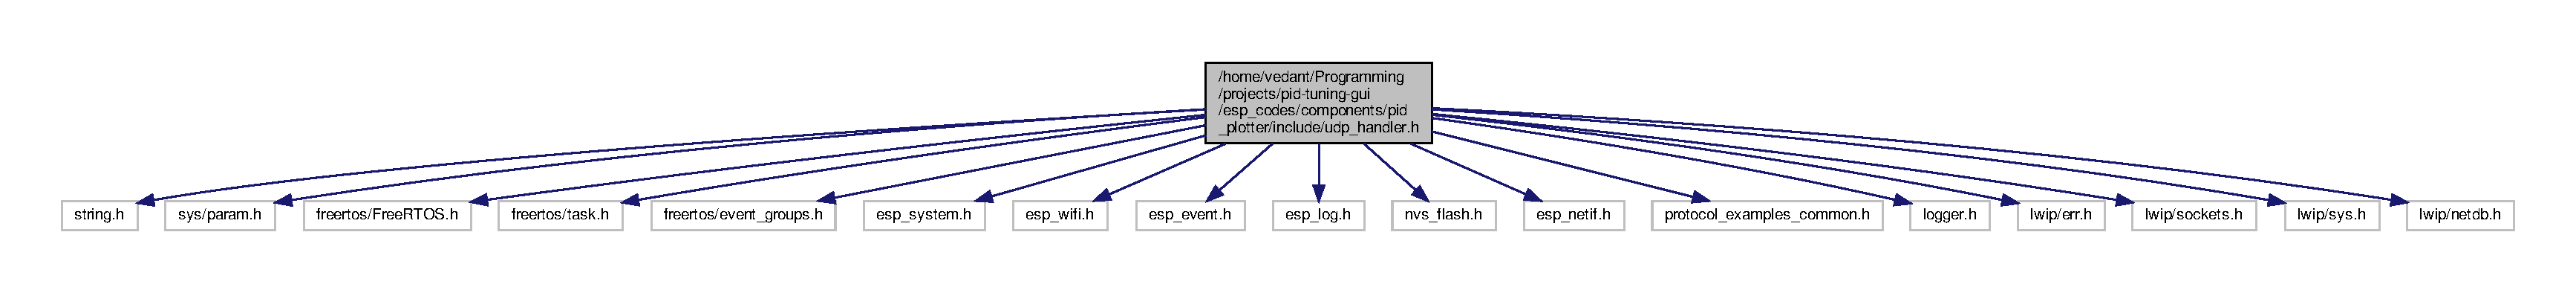
\includegraphics[width=350pt]{udp__handler_8h__incl}
\end{center}
\end{figure}
This graph shows which files directly or indirectly include this file\+:\nopagebreak
\begin{figure}[H]
\begin{center}
\leavevmode
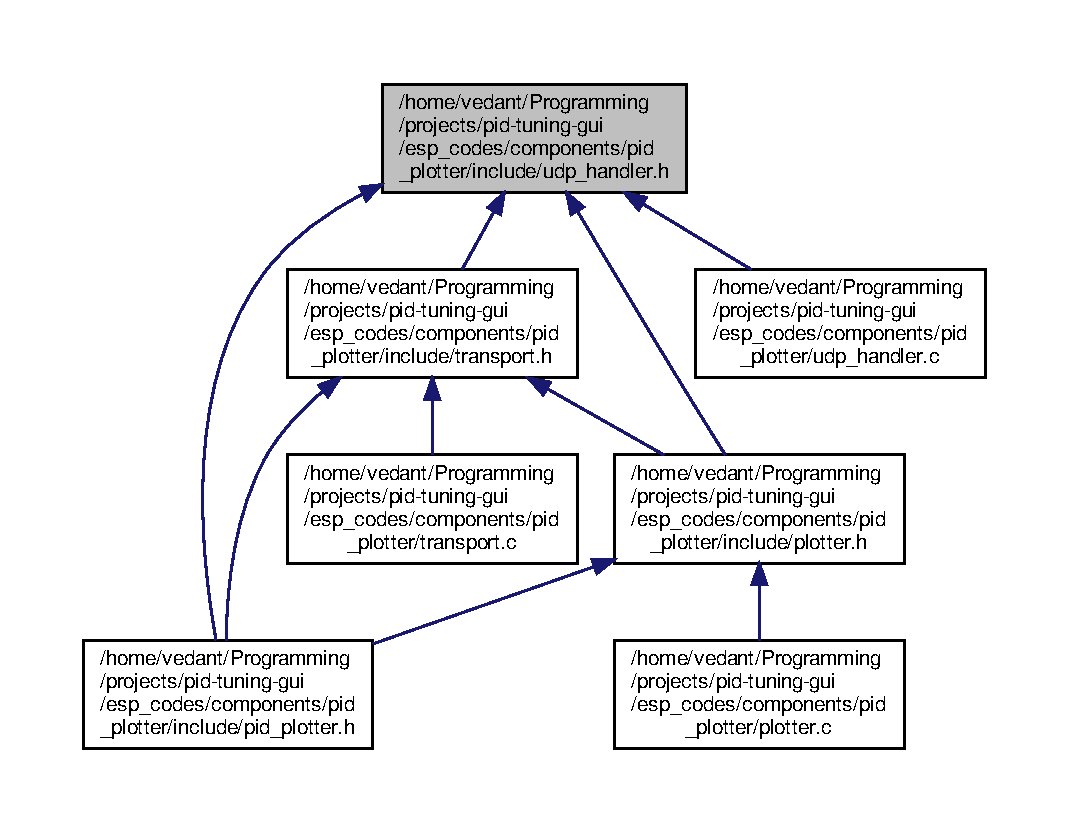
\includegraphics[width=350pt]{udp__handler_8h__dep__incl}
\end{center}
\end{figure}
\subsection*{Classes}
\begin{DoxyCompactItemize}
\item 
struct \hyperlink{structnetwork__data}{network\+\_\+data}
\end{DoxyCompactItemize}
\subsection*{Macros}
\begin{DoxyCompactItemize}
\item 
\#define \hyperlink{udp__handler_8h_a0755be366390c472fea523dda78961d3}{H\+O\+S\+T\+\_\+\+I\+P\+\_\+\+A\+D\+DR}~C\+O\+N\+F\+I\+G\+\_\+\+U\+D\+P\+\_\+\+I\+P\+\_\+\+A\+D\+D\+R\+E\+SS
\item 
\#define \hyperlink{udp__handler_8h_a614217d263be1fb1a5f76e2ff7be19a2}{P\+O\+RT}~C\+O\+N\+F\+I\+G\+\_\+\+U\+D\+P\+\_\+\+P\+O\+RT
\end{DoxyCompactItemize}
\subsection*{Functions}
\begin{DoxyCompactItemize}
\item 
void \hyperlink{udp__handler_8h_a412aa3402fc47e327861b48a04c3c08a}{network\+\_\+manager} (struct \hyperlink{structnetwork__data}{network\+\_\+data} $\ast$nm)
\begin{DoxyCompactList}\small\item\em Manages U\+DP connection to the server. \end{DoxyCompactList}\item 
int \hyperlink{udp__handler_8h_a7ddbd791c1d13c96db95eba36aae6145}{send\+\_\+data} (struct \hyperlink{structnetwork__data}{network\+\_\+data} $\ast$nm, char $\ast$payload)
\begin{DoxyCompactList}\small\item\em Sends data to the server through a U\+DP socket. \end{DoxyCompactList}\item 
char $\ast$ \hyperlink{udp__handler_8h_afe419fdd19f7194dcf9c9e6d00118224}{recieve\+\_\+data} (struct \hyperlink{structnetwork__data}{network\+\_\+data} $\ast$nm)
\begin{DoxyCompactList}\small\item\em Receives data from U\+DP server. \end{DoxyCompactList}\item 
void \hyperlink{udp__handler_8h_a3e138ed94c89bd74c249c9f4a1a4c642}{close\+\_\+network\+\_\+manager} (struct \hyperlink{structnetwork__data}{network\+\_\+data} $\ast$nm)
\begin{DoxyCompactList}\small\item\em Shutdown active connection, deallocate memory. \end{DoxyCompactList}\end{DoxyCompactItemize}


\subsection{Macro Definition Documentation}
\mbox{\Hypertarget{udp__handler_8h_a0755be366390c472fea523dda78961d3}\label{udp__handler_8h_a0755be366390c472fea523dda78961d3}} 
\index{udp\+\_\+handler.\+h@{udp\+\_\+handler.\+h}!H\+O\+S\+T\+\_\+\+I\+P\+\_\+\+A\+D\+DR@{H\+O\+S\+T\+\_\+\+I\+P\+\_\+\+A\+D\+DR}}
\index{H\+O\+S\+T\+\_\+\+I\+P\+\_\+\+A\+D\+DR@{H\+O\+S\+T\+\_\+\+I\+P\+\_\+\+A\+D\+DR}!udp\+\_\+handler.\+h@{udp\+\_\+handler.\+h}}
\subsubsection{\texorpdfstring{H\+O\+S\+T\+\_\+\+I\+P\+\_\+\+A\+D\+DR}{HOST\_IP\_ADDR}}
{\footnotesize\ttfamily \#define H\+O\+S\+T\+\_\+\+I\+P\+\_\+\+A\+D\+DR~C\+O\+N\+F\+I\+G\+\_\+\+U\+D\+P\+\_\+\+I\+P\+\_\+\+A\+D\+D\+R\+E\+SS}

\mbox{\Hypertarget{udp__handler_8h_a614217d263be1fb1a5f76e2ff7be19a2}\label{udp__handler_8h_a614217d263be1fb1a5f76e2ff7be19a2}} 
\index{udp\+\_\+handler.\+h@{udp\+\_\+handler.\+h}!P\+O\+RT@{P\+O\+RT}}
\index{P\+O\+RT@{P\+O\+RT}!udp\+\_\+handler.\+h@{udp\+\_\+handler.\+h}}
\subsubsection{\texorpdfstring{P\+O\+RT}{PORT}}
{\footnotesize\ttfamily \#define P\+O\+RT~C\+O\+N\+F\+I\+G\+\_\+\+U\+D\+P\+\_\+\+P\+O\+RT}



\subsection{Function Documentation}
\mbox{\Hypertarget{udp__handler_8h_a3e138ed94c89bd74c249c9f4a1a4c642}\label{udp__handler_8h_a3e138ed94c89bd74c249c9f4a1a4c642}} 
\index{udp\+\_\+handler.\+h@{udp\+\_\+handler.\+h}!close\+\_\+network\+\_\+manager@{close\+\_\+network\+\_\+manager}}
\index{close\+\_\+network\+\_\+manager@{close\+\_\+network\+\_\+manager}!udp\+\_\+handler.\+h@{udp\+\_\+handler.\+h}}
\subsubsection{\texorpdfstring{close\+\_\+network\+\_\+manager()}{close\_network\_manager()}}
{\footnotesize\ttfamily void close\+\_\+network\+\_\+manager (\begin{DoxyParamCaption}\item[{struct \hyperlink{structnetwork__data}{network\+\_\+data} $\ast$}]{nm }\end{DoxyParamCaption})}



Shutdown active connection, deallocate memory. 


\begin{DoxyParams}{Parameters}
{\em nm} & \hyperlink{structtcp__network__data}{tcp\+\_\+network\+\_\+data} struct which contains connection info \\
\hline
\end{DoxyParams}
\begin{DoxyReturn}{Returns}
void 
\end{DoxyReturn}
\mbox{\Hypertarget{udp__handler_8h_a412aa3402fc47e327861b48a04c3c08a}\label{udp__handler_8h_a412aa3402fc47e327861b48a04c3c08a}} 
\index{udp\+\_\+handler.\+h@{udp\+\_\+handler.\+h}!network\+\_\+manager@{network\+\_\+manager}}
\index{network\+\_\+manager@{network\+\_\+manager}!udp\+\_\+handler.\+h@{udp\+\_\+handler.\+h}}
\subsubsection{\texorpdfstring{network\+\_\+manager()}{network\_manager()}}
{\footnotesize\ttfamily void network\+\_\+manager (\begin{DoxyParamCaption}\item[{struct \hyperlink{structnetwork__data}{network\+\_\+data} $\ast$}]{nm }\end{DoxyParamCaption})}



Manages U\+DP connection to the server. 


\begin{DoxyParams}{Parameters}
{\em nm} & \hyperlink{structnetwork__data}{network\+\_\+data} struct which contains necessary data for a U\+DP connection \\
\hline
\end{DoxyParams}
\begin{DoxyReturn}{Returns}
void 
\end{DoxyReturn}
\mbox{\Hypertarget{udp__handler_8h_afe419fdd19f7194dcf9c9e6d00118224}\label{udp__handler_8h_afe419fdd19f7194dcf9c9e6d00118224}} 
\index{udp\+\_\+handler.\+h@{udp\+\_\+handler.\+h}!recieve\+\_\+data@{recieve\+\_\+data}}
\index{recieve\+\_\+data@{recieve\+\_\+data}!udp\+\_\+handler.\+h@{udp\+\_\+handler.\+h}}
\subsubsection{\texorpdfstring{recieve\+\_\+data()}{recieve\_data()}}
{\footnotesize\ttfamily char$\ast$ recieve\+\_\+data (\begin{DoxyParamCaption}\item[{struct \hyperlink{structnetwork__data}{network\+\_\+data} $\ast$}]{nm }\end{DoxyParamCaption})}



Receives data from U\+DP server. 


\begin{DoxyParams}{Parameters}
{\em nm} & \hyperlink{structnetwork__data}{network\+\_\+data} struct which contains connection info \\
\hline
\end{DoxyParams}
\begin{DoxyReturn}{Returns}
char array which contains data received 
\end{DoxyReturn}
\mbox{\Hypertarget{udp__handler_8h_a7ddbd791c1d13c96db95eba36aae6145}\label{udp__handler_8h_a7ddbd791c1d13c96db95eba36aae6145}} 
\index{udp\+\_\+handler.\+h@{udp\+\_\+handler.\+h}!send\+\_\+data@{send\+\_\+data}}
\index{send\+\_\+data@{send\+\_\+data}!udp\+\_\+handler.\+h@{udp\+\_\+handler.\+h}}
\subsubsection{\texorpdfstring{send\+\_\+data()}{send\_data()}}
{\footnotesize\ttfamily int send\+\_\+data (\begin{DoxyParamCaption}\item[{struct \hyperlink{structnetwork__data}{network\+\_\+data} $\ast$}]{nm,  }\item[{char $\ast$}]{payload }\end{DoxyParamCaption})}



Sends data to the server through a U\+DP socket. 


\begin{DoxyParams}{Parameters}
{\em nm} & A pointer to \hyperlink{structnetwork__data}{network\+\_\+data} struct \\
\hline
{\em payload} & char array which contains data to be sent \\
\hline
\end{DoxyParams}
\begin{DoxyReturn}{Returns}
int -\/ returns -\/1 if sending failed, number of bytes sent if successfully sent the data 
\end{DoxyReturn}

\hypertarget{json__handler_8c}{}\section{/home/vedant/\+Programming/projects/pid-\/tuning-\/gui/esp\+\_\+codes/components/pid\+\_\+plotter/json\+\_\+handler.c File Reference}
\label{json__handler_8c}\index{/home/vedant/\+Programming/projects/pid-\/tuning-\/gui/esp\+\_\+codes/components/pid\+\_\+plotter/json\+\_\+handler.\+c@{/home/vedant/\+Programming/projects/pid-\/tuning-\/gui/esp\+\_\+codes/components/pid\+\_\+plotter/json\+\_\+handler.\+c}}
{\ttfamily \#include \char`\"{}json\+\_\+handler.\+h\char`\"{}}\newline
Include dependency graph for json\+\_\+handler.\+c\+:\nopagebreak
\begin{figure}[H]
\begin{center}
\leavevmode
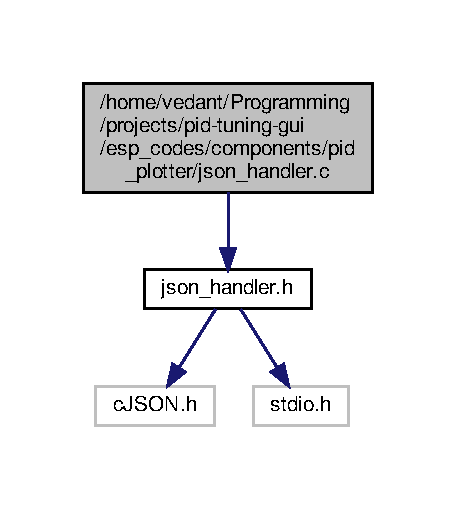
\includegraphics[width=219pt]{json__handler_8c__incl}
\end{center}
\end{figure}
\subsection*{Functions}
\begin{DoxyCompactItemize}
\item 
char $\ast$ \hyperlink{json__handler_8c_a229aa3d7fb017d31499a5e29b78b7f08}{create\+\_\+pid\+\_\+data\+\_\+to\+\_\+json} (float current, float error, float P, float I, float D)
\begin{DoxyCompactList}\small\item\em Converts P\+ID data to a json string. \end{DoxyCompactList}\item 
struct \hyperlink{structpid__const}{pid\+\_\+const} \hyperlink{json__handler_8c_a5a00fbe2cfe762fae40bd73932ddb072}{read\+\_\+pid\+\_\+data\+\_\+from\+\_\+json} (const char $\ast$data)
\begin{DoxyCompactList}\small\item\em Reads P\+ID constant data from a json formatted string. \end{DoxyCompactList}\end{DoxyCompactItemize}


\subsection{Function Documentation}
\mbox{\Hypertarget{json__handler_8c_a229aa3d7fb017d31499a5e29b78b7f08}\label{json__handler_8c_a229aa3d7fb017d31499a5e29b78b7f08}} 
\index{json\+\_\+handler.\+c@{json\+\_\+handler.\+c}!create\+\_\+pid\+\_\+data\+\_\+to\+\_\+json@{create\+\_\+pid\+\_\+data\+\_\+to\+\_\+json}}
\index{create\+\_\+pid\+\_\+data\+\_\+to\+\_\+json@{create\+\_\+pid\+\_\+data\+\_\+to\+\_\+json}!json\+\_\+handler.\+c@{json\+\_\+handler.\+c}}
\subsubsection{\texorpdfstring{create\+\_\+pid\+\_\+data\+\_\+to\+\_\+json()}{create\_pid\_data\_to\_json()}}
{\footnotesize\ttfamily char$\ast$ create\+\_\+pid\+\_\+data\+\_\+to\+\_\+json (\begin{DoxyParamCaption}\item[{float}]{current,  }\item[{float}]{error,  }\item[{float}]{P,  }\item[{float}]{I,  }\item[{float}]{D }\end{DoxyParamCaption})}



Converts P\+ID data to a json string. 


\begin{DoxyParams}{Parameters}
{\em current} & current value \\
\hline
{\em error} & error value, deviation of current from setpoint \\
\hline
{\em P} & Value of Proportional Gain (P) \\
\hline
{\em I} & Value of Integral Gain (I) \\
\hline
{\em D} & Value of Derivative Gain (D) \\
\hline
\end{DoxyParams}
\begin{DoxyReturn}{Returns}
char$\ast$ -\/ Json string of the data sent through parameters. 
\end{DoxyReturn}
\mbox{\Hypertarget{json__handler_8c_a5a00fbe2cfe762fae40bd73932ddb072}\label{json__handler_8c_a5a00fbe2cfe762fae40bd73932ddb072}} 
\index{json\+\_\+handler.\+c@{json\+\_\+handler.\+c}!read\+\_\+pid\+\_\+data\+\_\+from\+\_\+json@{read\+\_\+pid\+\_\+data\+\_\+from\+\_\+json}}
\index{read\+\_\+pid\+\_\+data\+\_\+from\+\_\+json@{read\+\_\+pid\+\_\+data\+\_\+from\+\_\+json}!json\+\_\+handler.\+c@{json\+\_\+handler.\+c}}
\subsubsection{\texorpdfstring{read\+\_\+pid\+\_\+data\+\_\+from\+\_\+json()}{read\_pid\_data\_from\_json()}}
{\footnotesize\ttfamily struct \hyperlink{structpid__const}{pid\+\_\+const} read\+\_\+pid\+\_\+data\+\_\+from\+\_\+json (\begin{DoxyParamCaption}\item[{const char $\ast$}]{data }\end{DoxyParamCaption})}



Reads P\+ID constant data from a json formatted string. 


\begin{DoxyParams}{Parameters}
{\em data} & Pointer to char array containging the json formatted string \\
\hline
\end{DoxyParams}
\begin{DoxyReturn}{Returns}
struct \hyperlink{structpid__const}{pid\+\_\+const} -\/ Returns a array of P\+ID constants, extracted from the json string 
\end{DoxyReturn}

\hypertarget{plotter_8c}{}\section{/home/vedant/\+Programming/projects/pid-\/tuning-\/gui/esp\+\_\+codes/components/pid\+\_\+plotter/plotter.c File Reference}
\label{plotter_8c}\index{/home/vedant/\+Programming/projects/pid-\/tuning-\/gui/esp\+\_\+codes/components/pid\+\_\+plotter/plotter.\+c@{/home/vedant/\+Programming/projects/pid-\/tuning-\/gui/esp\+\_\+codes/components/pid\+\_\+plotter/plotter.\+c}}
{\ttfamily \#include \char`\"{}plotter.\+h\char`\"{}}\newline
Include dependency graph for plotter.\+c\+:\nopagebreak
\begin{figure}[H]
\begin{center}
\leavevmode
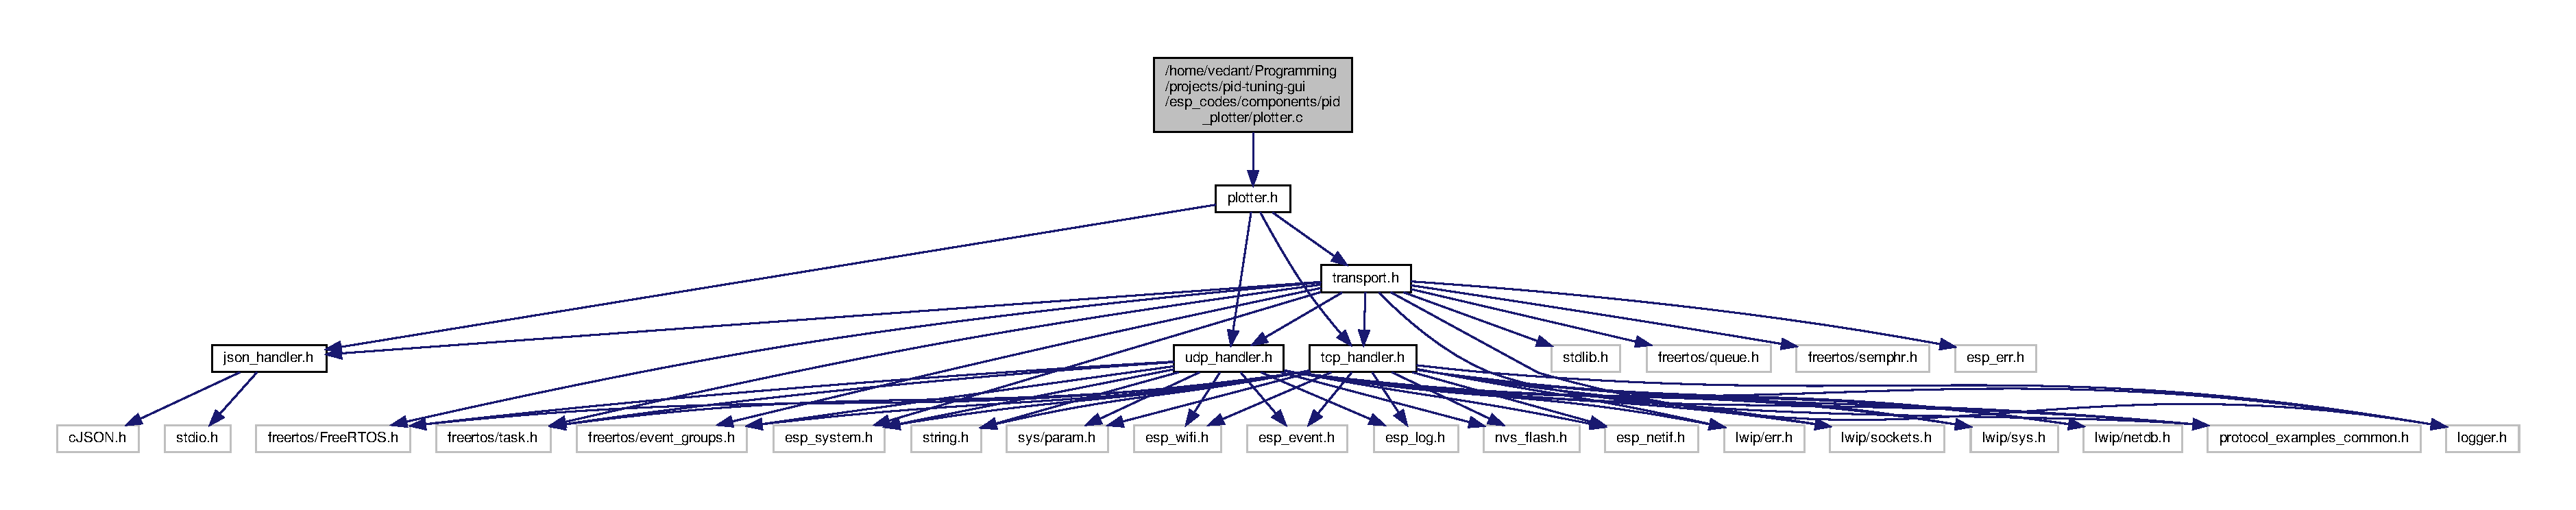
\includegraphics[width=350pt]{plotter_8c__incl}
\end{center}
\end{figure}
\subsection*{Functions}
\begin{DoxyCompactItemize}
\item 
void \hyperlink{plotter_8c_acc8c0bc33035955e5c765b474fb33ef1}{plotter} ()
\begin{DoxyCompactList}\small\item\em Wrapper function to run the plotter functionality on a separate core. \end{DoxyCompactList}\end{DoxyCompactItemize}


\subsection{Function Documentation}
\mbox{\Hypertarget{plotter_8c_acc8c0bc33035955e5c765b474fb33ef1}\label{plotter_8c_acc8c0bc33035955e5c765b474fb33ef1}} 
\index{plotter.\+c@{plotter.\+c}!plotter@{plotter}}
\index{plotter@{plotter}!plotter.\+c@{plotter.\+c}}
\subsubsection{\texorpdfstring{plotter()}{plotter()}}
{\footnotesize\ttfamily void plotter (\begin{DoxyParamCaption}{ }\end{DoxyParamCaption})}



Wrapper function to run the plotter functionality on a separate core. 


\hypertarget{tcp__handler_8c}{}\section{/home/vedant/\+Programming/projects/pid-\/tuning-\/gui/esp\+\_\+codes/components/pid\+\_\+plotter/tcp\+\_\+handler.c File Reference}
\label{tcp__handler_8c}\index{/home/vedant/\+Programming/projects/pid-\/tuning-\/gui/esp\+\_\+codes/components/pid\+\_\+plotter/tcp\+\_\+handler.\+c@{/home/vedant/\+Programming/projects/pid-\/tuning-\/gui/esp\+\_\+codes/components/pid\+\_\+plotter/tcp\+\_\+handler.\+c}}
{\ttfamily \#include \char`\"{}tcp\+\_\+handler.\+h\char`\"{}}\newline
Include dependency graph for tcp\+\_\+handler.\+c\+:
\nopagebreak
\begin{figure}[H]
\begin{center}
\leavevmode
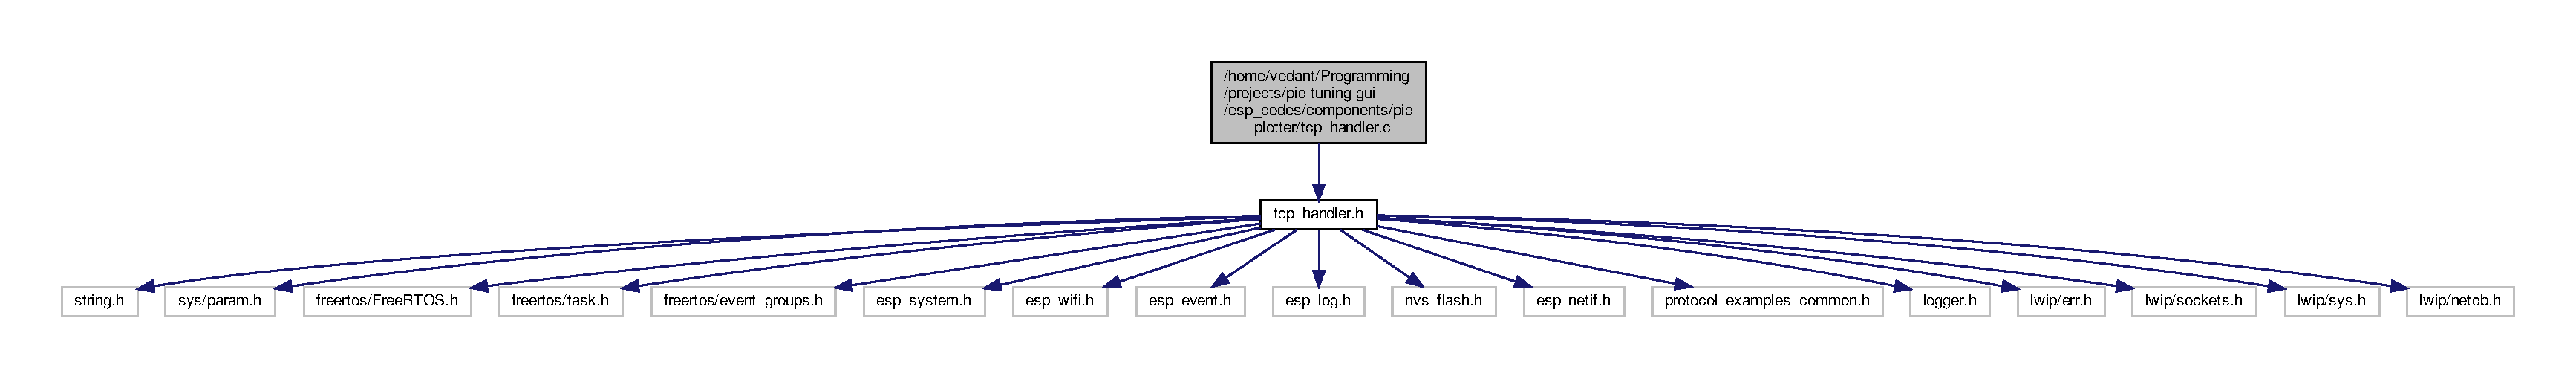
\includegraphics[width=350pt]{tcp__handler_8c__incl}
\end{center}
\end{figure}
\subsection*{Functions}
\begin{DoxyCompactItemize}
\item 
void \hyperlink{tcp__handler_8c_a6be7633691ba5c012155871a84ade82e}{tcp\+\_\+network\+\_\+manager} (struct \hyperlink{structtcp__network__data}{tcp\+\_\+network\+\_\+data} $\ast$nm)
\begin{DoxyCompactList}\small\item\em Manages T\+CP connection to the server. \end{DoxyCompactList}\item 
int \hyperlink{tcp__handler_8c_a0ca62b309e39660b29ee7605b099ee54}{tcp\+\_\+send\+\_\+data} (struct \hyperlink{structtcp__network__data}{tcp\+\_\+network\+\_\+data} $\ast$nm, char $\ast$payload)
\begin{DoxyCompactList}\small\item\em Sends data to the server through a T\+CP socket. \end{DoxyCompactList}\item 
char $\ast$ \hyperlink{tcp__handler_8c_ae58555e8930155fcea5b1d16915db87b}{tcp\+\_\+recieve\+\_\+data} (struct \hyperlink{structtcp__network__data}{tcp\+\_\+network\+\_\+data} $\ast$nm)
\begin{DoxyCompactList}\small\item\em Receives data from T\+CP server. \end{DoxyCompactList}\item 
void \hyperlink{tcp__handler_8c_a6d6a248c21ebfece9f52fa7b580fabb5}{tcp\+\_\+close\+\_\+network\+\_\+manager} (struct \hyperlink{structtcp__network__data}{tcp\+\_\+network\+\_\+data} $\ast$nm)
\begin{DoxyCompactList}\small\item\em Shutdown active connection, deallocate memory. \end{DoxyCompactList}\end{DoxyCompactItemize}


\subsection{Function Documentation}
\mbox{\Hypertarget{tcp__handler_8c_a6d6a248c21ebfece9f52fa7b580fabb5}\label{tcp__handler_8c_a6d6a248c21ebfece9f52fa7b580fabb5}} 
\index{tcp\+\_\+handler.\+c@{tcp\+\_\+handler.\+c}!tcp\+\_\+close\+\_\+network\+\_\+manager@{tcp\+\_\+close\+\_\+network\+\_\+manager}}
\index{tcp\+\_\+close\+\_\+network\+\_\+manager@{tcp\+\_\+close\+\_\+network\+\_\+manager}!tcp\+\_\+handler.\+c@{tcp\+\_\+handler.\+c}}
\subsubsection{\texorpdfstring{tcp\+\_\+close\+\_\+network\+\_\+manager()}{tcp\_close\_network\_manager()}}
{\footnotesize\ttfamily void tcp\+\_\+close\+\_\+network\+\_\+manager (\begin{DoxyParamCaption}\item[{struct \hyperlink{structtcp__network__data}{tcp\+\_\+network\+\_\+data} $\ast$}]{nm }\end{DoxyParamCaption})}



Shutdown active connection, deallocate memory. 


\begin{DoxyParams}{Parameters}
{\em nm} & \hyperlink{structtcp__network__data}{tcp\+\_\+network\+\_\+data} struct which contains connection info \\
\hline
\end{DoxyParams}
\begin{DoxyReturn}{Returns}
void 
\end{DoxyReturn}
\mbox{\Hypertarget{tcp__handler_8c_a6be7633691ba5c012155871a84ade82e}\label{tcp__handler_8c_a6be7633691ba5c012155871a84ade82e}} 
\index{tcp\+\_\+handler.\+c@{tcp\+\_\+handler.\+c}!tcp\+\_\+network\+\_\+manager@{tcp\+\_\+network\+\_\+manager}}
\index{tcp\+\_\+network\+\_\+manager@{tcp\+\_\+network\+\_\+manager}!tcp\+\_\+handler.\+c@{tcp\+\_\+handler.\+c}}
\subsubsection{\texorpdfstring{tcp\+\_\+network\+\_\+manager()}{tcp\_network\_manager()}}
{\footnotesize\ttfamily void tcp\+\_\+network\+\_\+manager (\begin{DoxyParamCaption}\item[{struct \hyperlink{structtcp__network__data}{tcp\+\_\+network\+\_\+data} $\ast$}]{nm }\end{DoxyParamCaption})}



Manages T\+CP connection to the server. 


\begin{DoxyParams}{Parameters}
{\em nm} & \hyperlink{structtcp__network__data}{tcp\+\_\+network\+\_\+data} struct which contains necessary data for a T\+CP connection \\
\hline
\end{DoxyParams}
\begin{DoxyReturn}{Returns}
void 
\end{DoxyReturn}
\mbox{\Hypertarget{tcp__handler_8c_ae58555e8930155fcea5b1d16915db87b}\label{tcp__handler_8c_ae58555e8930155fcea5b1d16915db87b}} 
\index{tcp\+\_\+handler.\+c@{tcp\+\_\+handler.\+c}!tcp\+\_\+recieve\+\_\+data@{tcp\+\_\+recieve\+\_\+data}}
\index{tcp\+\_\+recieve\+\_\+data@{tcp\+\_\+recieve\+\_\+data}!tcp\+\_\+handler.\+c@{tcp\+\_\+handler.\+c}}
\subsubsection{\texorpdfstring{tcp\+\_\+recieve\+\_\+data()}{tcp\_recieve\_data()}}
{\footnotesize\ttfamily char$\ast$ tcp\+\_\+recieve\+\_\+data (\begin{DoxyParamCaption}\item[{struct \hyperlink{structtcp__network__data}{tcp\+\_\+network\+\_\+data} $\ast$}]{nm }\end{DoxyParamCaption})}



Receives data from T\+CP server. 


\begin{DoxyParams}{Parameters}
{\em nm} & \hyperlink{structtcp__network__data}{tcp\+\_\+network\+\_\+data} struct which contains connection info \\
\hline
\end{DoxyParams}
\begin{DoxyReturn}{Returns}
char array which contains data received 
\end{DoxyReturn}
\mbox{\Hypertarget{tcp__handler_8c_a0ca62b309e39660b29ee7605b099ee54}\label{tcp__handler_8c_a0ca62b309e39660b29ee7605b099ee54}} 
\index{tcp\+\_\+handler.\+c@{tcp\+\_\+handler.\+c}!tcp\+\_\+send\+\_\+data@{tcp\+\_\+send\+\_\+data}}
\index{tcp\+\_\+send\+\_\+data@{tcp\+\_\+send\+\_\+data}!tcp\+\_\+handler.\+c@{tcp\+\_\+handler.\+c}}
\subsubsection{\texorpdfstring{tcp\+\_\+send\+\_\+data()}{tcp\_send\_data()}}
{\footnotesize\ttfamily int tcp\+\_\+send\+\_\+data (\begin{DoxyParamCaption}\item[{struct \hyperlink{structtcp__network__data}{tcp\+\_\+network\+\_\+data} $\ast$}]{nm,  }\item[{char $\ast$}]{payload }\end{DoxyParamCaption})}



Sends data to the server through a T\+CP socket. 


\begin{DoxyParams}{Parameters}
{\em nm} & A pointer to \hyperlink{structtcp__network__data}{tcp\+\_\+network\+\_\+data} struct \\
\hline
{\em payload} & char array which contains data to be sent \\
\hline
\end{DoxyParams}
\begin{DoxyReturn}{Returns}
int -\/ returns -\/1 if sending failed, number of bytes sent if successfully sent the data 
\end{DoxyReturn}

\hypertarget{transport_8c}{}\section{/home/vedant/\+Programming/projects/pid-\/tuning-\/gui/esp\+\_\+codes/components/pid\+\_\+plotter/transport.c File Reference}
\label{transport_8c}\index{/home/vedant/\+Programming/projects/pid-\/tuning-\/gui/esp\+\_\+codes/components/pid\+\_\+plotter/transport.\+c@{/home/vedant/\+Programming/projects/pid-\/tuning-\/gui/esp\+\_\+codes/components/pid\+\_\+plotter/transport.\+c}}
{\ttfamily \#include \char`\"{}transport.\+h\char`\"{}}\newline
Include dependency graph for transport.\+c\+:
\nopagebreak
\begin{figure}[H]
\begin{center}
\leavevmode
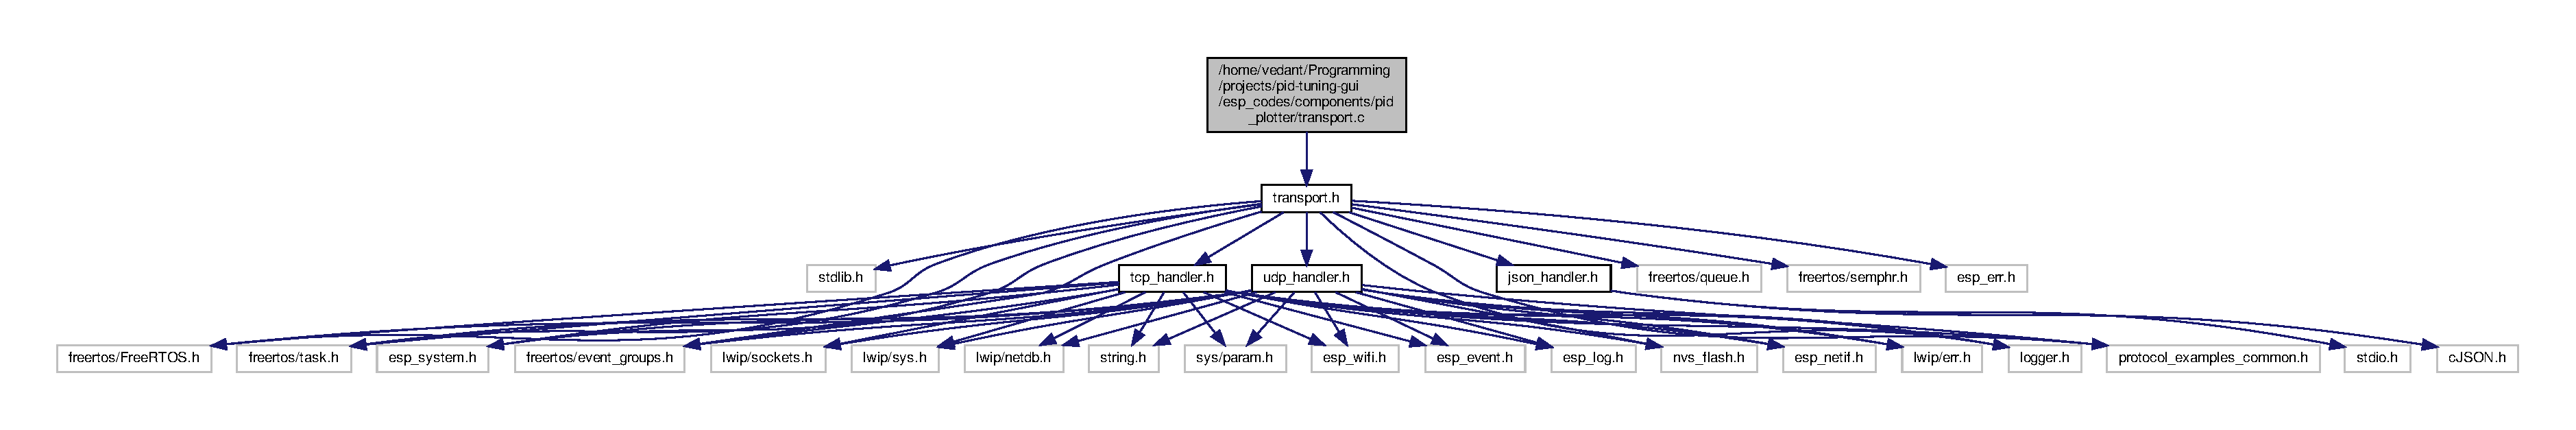
\includegraphics[width=350pt]{transport_8c__incl}
\end{center}
\end{figure}
\subsection*{Functions}
\begin{DoxyCompactItemize}
\item 
esp\+\_\+err\+\_\+t \hyperlink{transport_8c_a320afeaba56579760e7e3185a3d1fa02}{init\+\_\+queue} (void)
\begin{DoxyCompactList}\small\item\em Initialises message queue. \end{DoxyCompactList}\item 
void \hyperlink{transport_8c_a6afdab1f1ab02c6ed620949a7d32ffa4}{init\+\_\+transport} (void)
\begin{DoxyCompactList}\small\item\em Initialises transport, i.\+e. connect to wifi. \end{DoxyCompactList}\item 
esp\+\_\+err\+\_\+t \hyperlink{transport_8c_a3d23daa4cae5ba60d838c8a2b785462e}{send\+\_\+to\+\_\+queue} (struct \hyperlink{structpid__terms}{pid\+\_\+terms} pid\+\_\+data)
\begin{DoxyCompactList}\small\item\em Sends pid\+\_\+data struct to message queue. \end{DoxyCompactList}\item 
struct \hyperlink{structdata__recv}{data\+\_\+recv} \hyperlink{transport_8c_a3f717da7b4c254e710bbfd76625b15e4}{receive\+\_\+from\+\_\+queue} (void)
\begin{DoxyCompactList}\small\item\em Receive data from queue. \end{DoxyCompactList}\item 
void \hyperlink{transport_8c_a56e72500cb37fcbc087c3c3125ab7f8e}{pid\+\_\+transport} ()
\begin{DoxyCompactList}\small\item\em Handles U\+DP client, which sends \hyperlink{structpid__terms}{pid\+\_\+terms} received through message queue. \end{DoxyCompactList}\item 
void \hyperlink{transport_8c_acaba133d8c5e0cbadc4cfff68feca9fc}{pid\+\_\+const\+\_\+transport} ()
\begin{DoxyCompactList}\small\item\em Handles T\+CP client, which receives pid\+\_\+constants from server, and parses the data and stores it in a global struct pid\+\_\+const\+\_\+data. \end{DoxyCompactList}\item 
struct \hyperlink{structpid__const}{pid\+\_\+const} \hyperlink{transport_8c_aa37b5765ca807a54890c516c916e7e9b}{pid\+\_\+const\+\_\+read} ()
\begin{DoxyCompactList}\small\item\em Returns pid\+\_\+const\+\_\+data struct. Checks if the resource is blocked by mutex for writing or it is accessible, waits till pid\+\_\+const\+\_\+data is accessible and returns it. \end{DoxyCompactList}\end{DoxyCompactItemize}


\subsection{Function Documentation}
\mbox{\Hypertarget{transport_8c_a320afeaba56579760e7e3185a3d1fa02}\label{transport_8c_a320afeaba56579760e7e3185a3d1fa02}} 
\index{transport.\+c@{transport.\+c}!init\+\_\+queue@{init\+\_\+queue}}
\index{init\+\_\+queue@{init\+\_\+queue}!transport.\+c@{transport.\+c}}
\subsubsection{\texorpdfstring{init\+\_\+queue()}{init\_queue()}}
{\footnotesize\ttfamily esp\+\_\+err\+\_\+t init\+\_\+queue (\begin{DoxyParamCaption}\item[{void}]{ }\end{DoxyParamCaption})}



Initialises message queue. 

\begin{DoxyReturn}{Returns}
esp\+\_\+err\+\_\+t E\+S\+P\+\_\+\+OK -\/ if queue init sucessfully, E\+S\+P\+\_\+\+F\+A\+IL -\/ if queue init failed 
\end{DoxyReturn}
\mbox{\Hypertarget{transport_8c_a6afdab1f1ab02c6ed620949a7d32ffa4}\label{transport_8c_a6afdab1f1ab02c6ed620949a7d32ffa4}} 
\index{transport.\+c@{transport.\+c}!init\+\_\+transport@{init\+\_\+transport}}
\index{init\+\_\+transport@{init\+\_\+transport}!transport.\+c@{transport.\+c}}
\subsubsection{\texorpdfstring{init\+\_\+transport()}{init\_transport()}}
{\footnotesize\ttfamily void init\+\_\+transport (\begin{DoxyParamCaption}\item[{void}]{ }\end{DoxyParamCaption})}



Initialises transport, i.\+e. connect to wifi. 

\mbox{\Hypertarget{transport_8c_aa37b5765ca807a54890c516c916e7e9b}\label{transport_8c_aa37b5765ca807a54890c516c916e7e9b}} 
\index{transport.\+c@{transport.\+c}!pid\+\_\+const\+\_\+read@{pid\+\_\+const\+\_\+read}}
\index{pid\+\_\+const\+\_\+read@{pid\+\_\+const\+\_\+read}!transport.\+c@{transport.\+c}}
\subsubsection{\texorpdfstring{pid\+\_\+const\+\_\+read()}{pid\_const\_read()}}
{\footnotesize\ttfamily struct \hyperlink{structpid__const}{pid\+\_\+const} pid\+\_\+const\+\_\+read (\begin{DoxyParamCaption}{ }\end{DoxyParamCaption})}



Returns pid\+\_\+const\+\_\+data struct. Checks if the resource is blocked by mutex for writing or it is accessible, waits till pid\+\_\+const\+\_\+data is accessible and returns it. 

\begin{DoxyReturn}{Returns}
struct \hyperlink{structpid__const}{pid\+\_\+const} -\/ Returns pid\+\_\+const\+\_\+data, can be used to access Kp, Ki, Kd and current values 
\end{DoxyReturn}
\mbox{\Hypertarget{transport_8c_acaba133d8c5e0cbadc4cfff68feca9fc}\label{transport_8c_acaba133d8c5e0cbadc4cfff68feca9fc}} 
\index{transport.\+c@{transport.\+c}!pid\+\_\+const\+\_\+transport@{pid\+\_\+const\+\_\+transport}}
\index{pid\+\_\+const\+\_\+transport@{pid\+\_\+const\+\_\+transport}!transport.\+c@{transport.\+c}}
\subsubsection{\texorpdfstring{pid\+\_\+const\+\_\+transport()}{pid\_const\_transport()}}
{\footnotesize\ttfamily void pid\+\_\+const\+\_\+transport (\begin{DoxyParamCaption}{ }\end{DoxyParamCaption})}



Handles T\+CP client, which receives pid\+\_\+constants from server, and parses the data and stores it in a global struct pid\+\_\+const\+\_\+data. 

\mbox{\Hypertarget{transport_8c_a56e72500cb37fcbc087c3c3125ab7f8e}\label{transport_8c_a56e72500cb37fcbc087c3c3125ab7f8e}} 
\index{transport.\+c@{transport.\+c}!pid\+\_\+transport@{pid\+\_\+transport}}
\index{pid\+\_\+transport@{pid\+\_\+transport}!transport.\+c@{transport.\+c}}
\subsubsection{\texorpdfstring{pid\+\_\+transport()}{pid\_transport()}}
{\footnotesize\ttfamily void pid\+\_\+transport (\begin{DoxyParamCaption}{ }\end{DoxyParamCaption})}



Handles U\+DP client, which sends \hyperlink{structpid__terms}{pid\+\_\+terms} received through message queue. 

\mbox{\Hypertarget{transport_8c_a3f717da7b4c254e710bbfd76625b15e4}\label{transport_8c_a3f717da7b4c254e710bbfd76625b15e4}} 
\index{transport.\+c@{transport.\+c}!receive\+\_\+from\+\_\+queue@{receive\+\_\+from\+\_\+queue}}
\index{receive\+\_\+from\+\_\+queue@{receive\+\_\+from\+\_\+queue}!transport.\+c@{transport.\+c}}
\subsubsection{\texorpdfstring{receive\+\_\+from\+\_\+queue()}{receive\_from\_queue()}}
{\footnotesize\ttfamily struct \hyperlink{structdata__recv}{data\+\_\+recv} receive\+\_\+from\+\_\+queue (\begin{DoxyParamCaption}\item[{void}]{ }\end{DoxyParamCaption})}



Receive data from queue. 

\begin{DoxyReturn}{Returns}
struct \hyperlink{structdata__recv}{data\+\_\+recv} -\/ struct containing \hyperlink{structpid__terms}{pid\+\_\+terms} and esp\+\_\+err\+\_\+t as members. \hyperlink{structpid__terms}{pid\+\_\+terms} contains pid terms 
\end{DoxyReturn}
\mbox{\Hypertarget{transport_8c_a3d23daa4cae5ba60d838c8a2b785462e}\label{transport_8c_a3d23daa4cae5ba60d838c8a2b785462e}} 
\index{transport.\+c@{transport.\+c}!send\+\_\+to\+\_\+queue@{send\+\_\+to\+\_\+queue}}
\index{send\+\_\+to\+\_\+queue@{send\+\_\+to\+\_\+queue}!transport.\+c@{transport.\+c}}
\subsubsection{\texorpdfstring{send\+\_\+to\+\_\+queue()}{send\_to\_queue()}}
{\footnotesize\ttfamily esp\+\_\+err\+\_\+t send\+\_\+to\+\_\+queue (\begin{DoxyParamCaption}\item[{struct \hyperlink{structpid__terms}{pid\+\_\+terms}}]{pid\+\_\+data }\end{DoxyParamCaption})}



Sends pid\+\_\+data struct to message queue. 


\begin{DoxyParams}{Parameters}
{\em pid\+\_\+data} & \hyperlink{structpid__terms}{pid\+\_\+terms} struct contains pid values \\
\hline
\end{DoxyParams}
\begin{DoxyReturn}{Returns}
esp\+\_\+err\+\_\+t E\+S\+P\+\_\+\+OK -\/ if queue init sucessfully, E\+S\+P\+\_\+\+F\+A\+IL -\/ if queue init failed 
\end{DoxyReturn}

\hypertarget{udp__handler_8c}{}\section{/home/vedant/\+Programming/projects/pid-\/tuning-\/gui/esp\+\_\+codes/components/pid\+\_\+plotter/udp\+\_\+handler.c File Reference}
\label{udp__handler_8c}\index{/home/vedant/\+Programming/projects/pid-\/tuning-\/gui/esp\+\_\+codes/components/pid\+\_\+plotter/udp\+\_\+handler.\+c@{/home/vedant/\+Programming/projects/pid-\/tuning-\/gui/esp\+\_\+codes/components/pid\+\_\+plotter/udp\+\_\+handler.\+c}}
{\ttfamily \#include \char`\"{}udp\+\_\+handler.\+h\char`\"{}}\newline
Include dependency graph for udp\+\_\+handler.\+c\+:\nopagebreak
\begin{figure}[H]
\begin{center}
\leavevmode
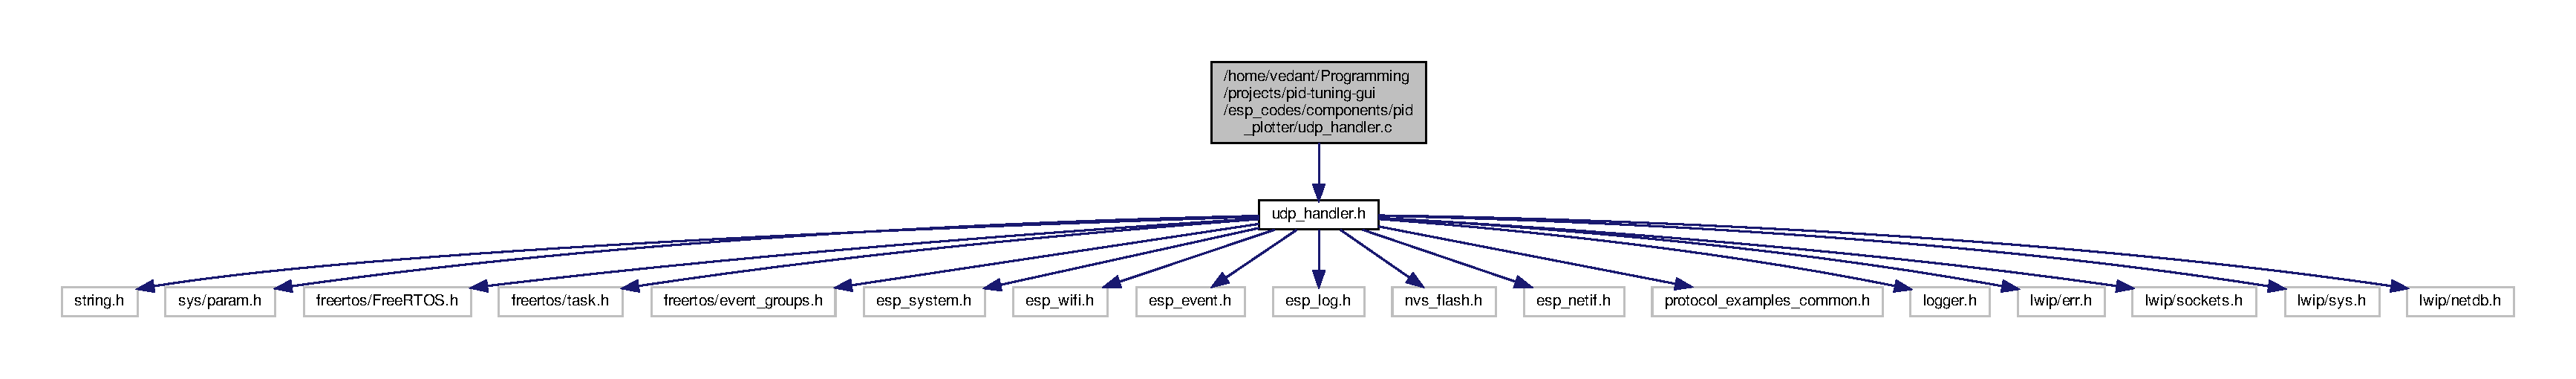
\includegraphics[width=350pt]{udp__handler_8c__incl}
\end{center}
\end{figure}
\subsection*{Functions}
\begin{DoxyCompactItemize}
\item 
void \hyperlink{udp__handler_8c_a412aa3402fc47e327861b48a04c3c08a}{network\+\_\+manager} (struct \hyperlink{structnetwork__data}{network\+\_\+data} $\ast$nm)
\begin{DoxyCompactList}\small\item\em Manages U\+DP connection to the server. \end{DoxyCompactList}\item 
int \hyperlink{udp__handler_8c_a7ddbd791c1d13c96db95eba36aae6145}{send\+\_\+data} (struct \hyperlink{structnetwork__data}{network\+\_\+data} $\ast$nm, char $\ast$payload)
\begin{DoxyCompactList}\small\item\em Sends data to the server through a U\+DP socket. \end{DoxyCompactList}\item 
char $\ast$ \hyperlink{udp__handler_8c_afe419fdd19f7194dcf9c9e6d00118224}{recieve\+\_\+data} (struct \hyperlink{structnetwork__data}{network\+\_\+data} $\ast$nm)
\begin{DoxyCompactList}\small\item\em Receives data from U\+DP server. \end{DoxyCompactList}\item 
void \hyperlink{udp__handler_8c_a3e138ed94c89bd74c249c9f4a1a4c642}{close\+\_\+network\+\_\+manager} (struct \hyperlink{structnetwork__data}{network\+\_\+data} $\ast$nm)
\begin{DoxyCompactList}\small\item\em Shutdown active connection, deallocate memory. \end{DoxyCompactList}\end{DoxyCompactItemize}


\subsection{Function Documentation}
\mbox{\Hypertarget{udp__handler_8c_a3e138ed94c89bd74c249c9f4a1a4c642}\label{udp__handler_8c_a3e138ed94c89bd74c249c9f4a1a4c642}} 
\index{udp\+\_\+handler.\+c@{udp\+\_\+handler.\+c}!close\+\_\+network\+\_\+manager@{close\+\_\+network\+\_\+manager}}
\index{close\+\_\+network\+\_\+manager@{close\+\_\+network\+\_\+manager}!udp\+\_\+handler.\+c@{udp\+\_\+handler.\+c}}
\subsubsection{\texorpdfstring{close\+\_\+network\+\_\+manager()}{close\_network\_manager()}}
{\footnotesize\ttfamily void close\+\_\+network\+\_\+manager (\begin{DoxyParamCaption}\item[{struct \hyperlink{structnetwork__data}{network\+\_\+data} $\ast$}]{nm }\end{DoxyParamCaption})}



Shutdown active connection, deallocate memory. 


\begin{DoxyParams}{Parameters}
{\em nm} & \hyperlink{structtcp__network__data}{tcp\+\_\+network\+\_\+data} struct which contains connection info \\
\hline
\end{DoxyParams}
\begin{DoxyReturn}{Returns}
void 
\end{DoxyReturn}
\mbox{\Hypertarget{udp__handler_8c_a412aa3402fc47e327861b48a04c3c08a}\label{udp__handler_8c_a412aa3402fc47e327861b48a04c3c08a}} 
\index{udp\+\_\+handler.\+c@{udp\+\_\+handler.\+c}!network\+\_\+manager@{network\+\_\+manager}}
\index{network\+\_\+manager@{network\+\_\+manager}!udp\+\_\+handler.\+c@{udp\+\_\+handler.\+c}}
\subsubsection{\texorpdfstring{network\+\_\+manager()}{network\_manager()}}
{\footnotesize\ttfamily void network\+\_\+manager (\begin{DoxyParamCaption}\item[{struct \hyperlink{structnetwork__data}{network\+\_\+data} $\ast$}]{nm }\end{DoxyParamCaption})}



Manages U\+DP connection to the server. 


\begin{DoxyParams}{Parameters}
{\em nm} & \hyperlink{structnetwork__data}{network\+\_\+data} struct which contains necessary data for a U\+DP connection \\
\hline
\end{DoxyParams}
\begin{DoxyReturn}{Returns}
void 
\end{DoxyReturn}
\mbox{\Hypertarget{udp__handler_8c_afe419fdd19f7194dcf9c9e6d00118224}\label{udp__handler_8c_afe419fdd19f7194dcf9c9e6d00118224}} 
\index{udp\+\_\+handler.\+c@{udp\+\_\+handler.\+c}!recieve\+\_\+data@{recieve\+\_\+data}}
\index{recieve\+\_\+data@{recieve\+\_\+data}!udp\+\_\+handler.\+c@{udp\+\_\+handler.\+c}}
\subsubsection{\texorpdfstring{recieve\+\_\+data()}{recieve\_data()}}
{\footnotesize\ttfamily char$\ast$ recieve\+\_\+data (\begin{DoxyParamCaption}\item[{struct \hyperlink{structnetwork__data}{network\+\_\+data} $\ast$}]{nm }\end{DoxyParamCaption})}



Receives data from U\+DP server. 


\begin{DoxyParams}{Parameters}
{\em nm} & \hyperlink{structnetwork__data}{network\+\_\+data} struct which contains connection info \\
\hline
\end{DoxyParams}
\begin{DoxyReturn}{Returns}
char array which contains data received 
\end{DoxyReturn}
\mbox{\Hypertarget{udp__handler_8c_a7ddbd791c1d13c96db95eba36aae6145}\label{udp__handler_8c_a7ddbd791c1d13c96db95eba36aae6145}} 
\index{udp\+\_\+handler.\+c@{udp\+\_\+handler.\+c}!send\+\_\+data@{send\+\_\+data}}
\index{send\+\_\+data@{send\+\_\+data}!udp\+\_\+handler.\+c@{udp\+\_\+handler.\+c}}
\subsubsection{\texorpdfstring{send\+\_\+data()}{send\_data()}}
{\footnotesize\ttfamily int send\+\_\+data (\begin{DoxyParamCaption}\item[{struct \hyperlink{structnetwork__data}{network\+\_\+data} $\ast$}]{nm,  }\item[{char $\ast$}]{payload }\end{DoxyParamCaption})}



Sends data to the server through a U\+DP socket. 


\begin{DoxyParams}{Parameters}
{\em nm} & A pointer to \hyperlink{structnetwork__data}{network\+\_\+data} struct \\
\hline
{\em payload} & char array which contains data to be sent \\
\hline
\end{DoxyParams}
\begin{DoxyReturn}{Returns}
int -\/ returns -\/1 if sending failed, number of bytes sent if successfully sent the data 
\end{DoxyReturn}

%--- End generated contents ---

% Index
\backmatter
\newpage
\phantomsection
\clearemptydoublepage
\addcontentsline{toc}{chapter}{Index}
\printindex

\end{document}
